\documentclass[a4paper,12pt,twoside]{memoir}

% Castellano
\usepackage[spanish,es-tabla]{babel}
\selectlanguage{spanish}
\usepackage[utf8]{inputenc}
\usepackage[T1]{fontenc}
\usepackage{lmodern} % Scalable font
\usepackage{microtype}
\usepackage{placeins}

\RequirePackage{booktabs}
\RequirePackage[table]{xcolor}
\RequirePackage{xtab}
\RequirePackage{multirow}
\usepackage{graphicx}
\usepackage{float}
\usepackage{lscape}
\usepackage{multicol}

% Links
\usepackage[colorlinks]{hyperref}
\hypersetup{
	allcolors = {red}
}

% Ecuaciones
\usepackage{amsmath}

% Rutas de fichero / paquete
\newcommand{\ruta}[1]{{\sffamily #1}}

% Párrafos
\nonzeroparskip

% Huérfanas y viudas
\widowpenalty100000
\clubpenalty100000

% Evitar solapes en el header
\nouppercaseheads

% Imagenes
\usepackage{graphicx}
\newcommand{\imagen}[2]{
	\begin{figure}[!h]
		\centering
		\includegraphics[width=0.9\textwidth]{#1}
		\caption{#2}\label{fig:#1}
	\end{figure}
	\FloatBarrier
}

\newcommand{\imagenflotante}[2]{
	\begin{figure}%[!h]
		\centering
		\includegraphics[width=0.9\textwidth]{#1}
		\caption{#2}\label{fig:#1}
	\end{figure}
}



% El comando \figura nos permite insertar figuras comodamente, y utilizando
% siempre el mismo formato. Los parametros son:
% 1 -> Porcentaje del ancho de página que ocupará la figura (de 0 a 1)
% 2 --> Fichero de la imagen
% 3 --> Texto a pie de imagen
% 4 --> Etiqueta (label) para referencias
% 5 --> Opciones que queramos pasarle al \includegraphics
% 6 --> Opciones de posicionamiento a pasarle a \begin{figure}
\newcommand{\figuraConPosicion}[6]{%
  \setlength{\anchoFloat}{#1\textwidth}%
  \addtolength{\anchoFloat}{-4\fboxsep}%
  \setlength{\anchoFigura}{\anchoFloat}%
  \begin{figure}[#6]
    \begin{center}%
      \Ovalbox{%
        \begin{minipage}{\anchoFloat}%
          \begin{center}%
            \includegraphics[width=\anchoFigura,#5]{#2}%
            \caption{#3}%
            \label{#4}%
          \end{center}%
        \end{minipage}
      }%
    \end{center}%
  \end{figure}%
}

%
% Comando para incluir imágenes en formato apaisado (sin marco).
\newcommand{\figuraApaisadaSinMarco}[5]{%
  \begin{figure}%
    \begin{center}%
    \includegraphics[angle=90,height=#1\textheight,#5]{#2}%
    \caption{#3}%
    \label{#4}%
    \end{center}%
  \end{figure}%
}
% Para las tablas
\newcommand{\otoprule}{\midrule [\heavyrulewidth]}
%
% Nuevo comando para tablas pequeñas (menos de una página).
\newcommand{\tablaSmall}[5]{%
 \begin{table}
  \begin{center}
   \rowcolors {2}{gray!35}{}
   \begin{tabular}{#2}
    \toprule
    #4
    \otoprule
    #5
    \bottomrule
   \end{tabular}
   \caption{#1}
   \label{tabla:#3}
  \end{center}
 \end{table}
}

%
% Nuevo comando para tablas pequeñas (menos de una página).
\newcommand{\tablaSmallSinColores}[5]{%
 \begin{table}[H]
  \begin{center}
   \begin{tabular}{#2}
    \toprule
    #4
    \otoprule
    #5
    \bottomrule
   \end{tabular}
   \caption{#1}
   \label{tabla:#3}
  \end{center}
 \end{table}
}

\newcommand{\tablaApaisadaSmall}[5]{%
\begin{landscape}
  \begin{table}
   \begin{center}
    \rowcolors {2}{gray!35}{}
    \begin{tabular}{#2}
     \toprule
     #4
     \otoprule
     #5
     \bottomrule
    \end{tabular}
    \caption{#1}
    \label{tabla:#3}
   \end{center}
  \end{table}
\end{landscape}
}

%
% Nuevo comando para tablas grandes con cabecera y filas alternas coloreadas en gris.
\newcommand{\tabla}[6]{%
  \begin{center}
    \tablefirsthead{
      \toprule
      #5
      \otoprule
    }
    \tablehead{
      \multicolumn{#3}{l}{\small\sl continúa desde la página anterior}\\
      \toprule
      #5
      \otoprule
    }
    \tabletail{
      \hline
      \multicolumn{#3}{r}{\small\sl continúa en la página siguiente}\\
    }
    \tablelasttail{
      \hline
    }
    \bottomcaption{#1}
    \rowcolors {2}{gray!35}{}
    \begin{xtabular}{#2}
      #6
      \bottomrule
    \end{xtabular}
    \label{tabla:#4}
  \end{center}
}

%
% Nuevo comando para tablas grandes con cabecera.
\newcommand{\tablaSinColores}[6]{%
  \begin{center}
    \tablefirsthead{
      \toprule
      #5
      \otoprule
    }
    \tablehead{
      \multicolumn{#3}{l}{\small\sl continúa desde la página anterior}\\
      \toprule
      #5
      \otoprule
    }
    \tabletail{
      \hline
      \multicolumn{#3}{r}{\small\sl continúa en la página siguiente}\\
    }
    \tablelasttail{
      \hline
    }
    \bottomcaption{#1}
    \begin{xtabular}{#2}
      #6
      \bottomrule
    \end{xtabular}
    \label{tabla:#4}
  \end{center}
}

%
% Nuevo comando para tablas grandes sin cabecera.
\newcommand{\tablaSinCabecera}[5]{%
  \begin{center}
    \tablefirsthead{
      \toprule
    }
    \tablehead{
      \multicolumn{#3}{l}{\small\sl continúa desde la página anterior}\\
      \hline
    }
    \tabletail{
      \hline
      \multicolumn{#3}{r}{\small\sl continúa en la página siguiente}\\
    }
    \tablelasttail{
      \hline
    }
    \bottomcaption{#1}
  \begin{xtabular}{#2}
    #5
   \bottomrule
  \end{xtabular}
  \label{tabla:#4}
  \end{center}
}



\definecolor{cgoLight}{HTML}{EEEEEE}
\definecolor{cgoExtralight}{HTML}{FFFFFF}

%
% Nuevo comando para tablas grandes sin cabecera.
\newcommand{\tablaSinCabeceraConBandas}[5]{%
  \begin{center}
    \tablefirsthead{
      \toprule
    }
    \tablehead{
      \multicolumn{#3}{l}{\small\sl continúa desde la página anterior}\\
      \hline
    }
    \tabletail{
      \hline
      \multicolumn{#3}{r}{\small\sl continúa en la página siguiente}\\
    }
    \tablelasttail{
      \hline
    }
    \bottomcaption{#1}
    \rowcolors[]{1}{cgoExtralight}{cgoLight}

  \begin{xtabular}{#2}
    #5
   \bottomrule
  \end{xtabular}
  \label{tabla:#4}
  \end{center}
}


\graphicspath{ {./img/} }

% Capítulos
\chapterstyle{bianchi}
\newcommand{\capitulo}[2]{
	\setcounter{chapter}{#1}
	\setcounter{section}{0}
	\chapter*{#2}
	\addcontentsline{toc}{chapter}{#1. #2}
	\markboth{#2}{#2}
}

% Apéndices
\renewcommand{\appendixname}{Apéndice}
\renewcommand*\cftappendixname{\appendixname}

\newcommand{\apendice}[1]{
	%\renewcommand{\thechapter}{A}
	\chapter{#1}
}

\renewcommand*\cftappendixname{\appendixname\ }

% Formato de portada
\makeatletter
\usepackage{xcolor}
\newcommand{\tutor}[1]{\def\@tutor{#1}}
\newcommand{\course}[1]{\def\@course{#1}}
\definecolor{cpardoBox}{HTML}{E6E6FF}
\def\maketitle{
  \null
  \thispagestyle{empty}
  % Cabecera ----------------
\begin{center}%
	{\noindent\Huge Universidades de Burgos, León y Valladolid}\vspace{.5cm}%
	
	{\noindent\Large Máster universitario}\vspace{.5cm}%
	
	{\noindent\Huge \textbf{Inteligencia de Negocio y Big~Data en Entornos Seguros}}\vspace{.5cm}%
\end{center}%

\begin{center}%
	
\includegraphics[height=3cm]{img/escudoUBU} \hspace{1cm}
	
\includegraphics[height=3cm]{img/escudoUVA} \hspace{1cm}
	
\includegraphics[height=3cm]{img/escudoULE} \vspace{1cm}%
\end{center}%

  \vfill
  % Título proyecto y escudo informática ----------------
  \colorbox{cpardoBox}{%
    \begin{minipage}{.9\textwidth}
      \vspace{.5cm}\Large
      \begin{center}
      \textbf{TFM del Máster Inteligencia de Negocio y Big Data en Entornos Seguros}\vspace{.6cm}\\
      \textbf{\LARGE\@title{}}
      \end{center}
      \vspace{.2cm}
    \end{minipage}

  }%
  \hfill
  \vfill
  % Datos de alumno, curso y tutores ------------------
  \begin{center}%
  {%
    \noindent\LARGE
    Presentado por \@author{}\\ 
    en Universidad de Burgos --- \@date{}\\
    Tutor: \@tutor{}\\
  }%
  \end{center}%
  \null
  \cleardoublepage
  }
\makeatother

\newcommand{\nombre}{Daniel González Alonso} %%% cambio de comando

% Datos de portada
\title{título del TFM}
\author{\nombre}
\tutor{Ángel Manuel Guerrero}
\date{\today}

\begin{document}

\maketitle


\newpage\null\thispagestyle{empty}\newpage


%%%%%%%%%%%%%%%%%%%%%%%%%%%%%%%%%%%%%%%%%%%%%%%%%%%%%%%%%%%%%%%%%%%%%%%%%%%%%%%%%%%%%%%%
\thispagestyle{empty}


\noindent
\begin{center}%
	{\noindent\Huge Universidades de Burgos, León y Valladolid}\vspace{.5cm}%
	
\begin{center}%
	
\includegraphics[height=3cm]{img/escudoUBU} \hspace{1cm}
	
\includegraphics[height=3cm]{img/escudoUVA} \hspace{1cm}
	
\includegraphics[height=3cm]{img/escudoULE} \vspace{1cm}%
\end{center}%

	{\noindent\Large \textbf{Máster universitario en Inteligencia de Negocio y Big~Data en Entornos Seguros}}\vspace{.5cm}%
\end{center}%



\noindent D. Ángel Manuel Guerrero Higueras, profesor del departamento de nombre departamento, área de nombre área.

\noindent Expone:

\noindent Que el alumno D. \nombre, con DNI 71178522P, ha realizado el Trabajo final de Máster en Inteligencia de Negocio y Big Data en Entornos Seguros 
          titulado título de TFM. 

\noindent Y que dicho trabajo ha sido realizado por el alumno bajo la dirección del que suscribe, en virtud de lo cual se autoriza su presentación y defensa.

\begin{center} %\large
En Burgos, {\large \today}
\end{center}

\vfill\vfill\vfill

% Author and supervisor
\begin{minipage}{0.45\textwidth}
\begin{flushleft} %\large
Vº. Bº. del Tutor:\\[2cm]
D. nombre tutor
\end{flushleft}
\end{minipage}
\hfill
\begin{minipage}{0.45\textwidth}
\begin{flushleft} %\large
Vº. Bº. del co-tutor:\\[2cm]
D. nombre co-tutor
\end{flushleft}
\end{minipage}
\hfill

\vfill

% para casos con solo un tutor comentar lo anterior
% y descomentar lo siguiente
%Vº. Bº. del Tutor:\\[2cm]
%D. nombre tutor


\newpage\null\thispagestyle{empty}\newpage




\frontmatter

% Abstract en castellano
\renewcommand*\abstractname{Resumen}
\begin{abstract}
En este primer apartado se hace una \textbf{breve} presentación del tema que se aborda en el proyecto.
\end{abstract}

\renewcommand*\abstractname{Descriptores}
\begin{abstract}
Palabras separadas por comas que identifiquen el contenido del proyecto Ej: servidor web, buscador de vuelos, android \ldots
\end{abstract}

\clearpage

% Abstract en inglés
\renewcommand*\abstractname{Abstract}
\begin{abstract}
A \textbf{brief} presentation of the topic addressed in the project.
\end{abstract}

\renewcommand*\abstractname{Keywords}
\begin{abstract}
keywords separated by commas.
\end{abstract}

\clearpage

% Indices
\tableofcontents

\clearpage

\listoffigures

\clearpage

\listoftables
\clearpage

\mainmatter

\addcontentsline{toc}{part}{Memoria}
\part*{Memoria}

\capitulo{1}{Introducción}

%Descripción del contenido del trabajo y del estructura de la memoria y del resto de materiales entregados.

El turismo es una de las actividades económicas más importantes de España, en 2019 suponía el 12,4\% del PIB del país, siendo el tercer país más visitado del mundo. Con la pandemia de COVID-19 el sector turístico se vio gravemente afectado por las restricciones de movilidad y el propio temor a la enfermedad. En la actualidad este sector todavía no ha recuperado los niveles previos a la pandemia. Si en 2019 se recibieron 83,5 millones de turistas, en 2021 esa cifra ha sido aproximadamente de 31,2 millones \cite{turismo_espana}.

En el caso de Valladolid en concreto, esta ciudad no partía de una situación ventajosa en comparación con otras ciudades de España, ubicándose en la zona media-baja de la tabla. Y al igual que el resto del país, la pandemia ha reducido el número de visitantes: la provincia has pasado de unos 51000 en 2019 a aproximadamente 33000 en 2021 de acuerdo al INE. 

Para recuperar los niveles de turismo previos (y seguir aumentándolos) es necesario potenciar el turismo, y uno de los posibles medios que se pueden aprovechar es internet, y en concreto las redes sociales. Saber explotar la información de las redes sociales puede tener una influencia enorme a la hora de mejorar el número de visitantes que pueda tener una ciudad. Pero abordar esta tarea es una asunto complicado.

Con la aparición y popularización de las redes sociales, cada vez más gente comparte los lugares que visita y sus opiniones. Las publicaciones que hace la gente en estas plataformas ayudan a otras personas a descubrir nuevas experiencias y lugares que visitar. También permite a las personas conocer más en detalle aquellos sitios a los que planea viajar. Por otro lado, todos estos contenidos generados por los usuarios son una fuente de información incalculable para todas aquellas empresas que están buscando mejorar sus productos vacacionales.

Una de las redes sociales más usadas en la actualidad es Instagram. Esta red social permite compartir publicaciones principalmente en forma de imagen o vídeo. La forma en que se muestra el contenido en esta red social la hace ideal para compartir lugares visitados o experiencias vividas, y aunque no sea el único tipo de publicaciones que se comparten en esta red social, si que es bastante común encontrarlo. Es por ello que los efectos que puede tener esta red social a la hora de difundir el potencial turístico que tiene una ubicación son muy importantes.

Cuando se llevan a cabo búsquedas en Instagram, las publicaciones que se muestran se basan en tres criterios, la cadena de búsqueda, los cuentas y hashtags que se siguen o visita y la popularidad de las publicaciones encontradas. Un problema que tiene esta forma de mostrar las publicaciones es que si se pretende hacer turismo a un lugar lejano, es posible que ninguno de tus contactos tenga influencia en los resultados, y es más que probable que Instagram tan solo muestre las publicaciones más populares del destino que estás buscando.

Es por ello que en este trabajo se pretende investigar el posible uso de reconocimientos de imágenes y análisis de sentimiento en las publicaciones de Instagram para facilitar el descubrimiento de actividades y lugares recomendables en Valladolid.

\section{Organización de la memoria}
La memoria se encuentra dividida en los siguientes capítulos:

\begin{enumerate}
    \item Introducción: presentación del proyecto y la relación del turismo con las redes sociales.
    \item Objetivos del proyecto: se presentan los distintos objetivos que se buscan cumplir con el desarrollo del proyecto.
    \item Conceptos teóricos: se introducen los conceptos teóricos necesarios para compresión de la memoria.
    \item Técnicas y herramientas: en este aparatado se busca enumerar y describir las múltiples herramientas, servicios, librerías y APIs empleadas para el desarrollo del proyecto.
    \item Aspectos relevantes del desarrollo del proyecto
    \item Trabajos relacionados: Estado del arte del proyecto.
    \item Conclusiones y Líneas de trabajo futuras
\end{enumerate}

\section{Organización de los apéndices}

\capitulo{2}{Objetivos del proyecto}

En este apartado se exponen los distintos objetivos que se pretenden satisfacer en el proyecto actual. Estos objetivos se han dividido en tres tipos: generales, técnicos y personales, los cuales se describen a continuación.

\section{Objetivos generales}

Los objetivos principales planteados para el proyecto son los siguientes:

\begin{itemize}
    \item Conocer el estado del arte, investigando artículos que ya hayan sido realizados en relación a la recomendación de publicaciones o lugares donde hacer turismo en base a contenido de redes sociales.
    \item Desarrollar el software necesario para descargar publicaciones de Instagram y su posterior almacenamiento.
    \item Usar algún servicio de reconocimiento de imágenes para llevar a cabo análisis de sentimiento sobre las publicaciones, así como la extracción de información relativa a las personas presentes en la imagen, como su edad o género.
    \item Implementar o usar algún medio para llevar a cabo la visualización y filtrado de los datos de forma sencilla.
\end{itemize}

\section{Objetivos técnicos}

En base a los objetivos anteriores se plantean los siguientes requerimientos técnicos:

\begin{itemize}
    \item Se busca el empleo de herramientas en la nube para el alojamiento y procesamiento de los datos.
    \item El desarrollo del proyecto no ha de suponer ningún coste, por ello se pretende usar software libre, herramientas gratuitas o herramientas que tengan un periodo de prueba lo suficientemente extenso como para poder desarrollar el proyecto sin complicaciones.
    \item Para la visualización de los datos se busca desarrollar un cuadro de mandos con alguna herramienta o servicio ya existente.
\end{itemize}

\section{Objetivos personales}

Entre los objetivos personales que se buscan satisfacer con este proyecto se encuentran los siguientes:

\begin{itemize}
    \item Familiarizarse con el uso de herramientas y servicios populares de computación en la nube.
    \item Ampliar mis conocimientos del lenguaje de programación Python así como aprender a usar nuevas librerías e interfaces de programación.
    \item Poner en práctica mis conocimientos sobre cuadros de mando, profundizando en el uso de herramientas utilizadas a lo largo del máster o aprendiendo a usar otras nuevas.
    \item Mejorar mis conocimientos sobre almacenamiento y procesado de grandes cantidades de datos.
\end{itemize}

\capitulo{3}{Conceptos teóricos}

En este apartado se presentan los distintos conceptos teóricos necesarios para la correcta comprensión del proyecto.

\section{Emoción y Sentimiento}

A pesar de que en el lenguaje popular en muchas ocasiones se usan ambas palabras de forma equivalente, no lo son. Las emociones y los sentimientos representan dos conceptos distintos aunque relacionados.

Por un lado, las emociones son un conjunto de reacciones neurofisiológicas que sufre un individuo al ser expuesto a algún objeto, lugar, persona, suceso o idea. Las emociones son transitorias, se dan de forma inconsciente y espontánea. En múltiples ocasiones las emociones son el origen de los cambios en la motivación y el comportamiento de los individuos. En ocasiones se dividen las emociones entre primarias o básicas y secundarias, siendo las 4 emociones primarias el miedo, la tristeza, el enfado y la alegría \cite{psicoemocionat}.

Por otro lado, los sentimientos son un estado afectivo que se genera a partir de una emoción \cite{psicoonline}. En el sentimiento interviene tanto la reacción neurofisiológica como un componente cognitivo. Esto significa que mientras que la emoción se daba de forma instintiva, en el sentimiento interviene un razonamiento que lo hace más duradero.

En resumen, las principales diferencias entre emoción y pensamiento radican en:
\begin{enumerate}
    \item Mientras que las emociones duran poco tiempo los sentimientos son duraderos.
    \item La emoción precede al sentimiento.
    \item Los sentimientos se producen instintivamente mientras que en los sentimientos interviene el pensamiento, el cual es afectado por la experiencia previa del individuo, características subjetivas, etc.
\end{enumerate}

\section{Análisis de Emociones y de Sentimientos}

Al igual que sucedía en el apartado anterior, los conceptos de análisis de emoción y de sentimiento a pesar de parecer similares no lo son.

Primero, el análisis de emociones busca descubrir la reacción que puede tener un individuo ante cierto estímulo. Como se comentó en el anteriormente, las emociones en muchas ocasiones son el motivo de las acciones de las personas, con lo que conocer si una persona se encuentra aburrida, contenta o enfadada puede ser de utilidad para dar una respuesta adecuada.

Por otro lado, el análisis de sentimiento no busca descubrir que emoción en particular es expresada por los usuarios, si no más bien conocer si la respuesta de un individuo es positiva o negativa, lo que se suele conocer como polaridad (en ocasiones también se incluye la neutralidad) \cite{analyticssteps}. Ejemplos de este tipo de análisis pueden ser el conocer el éxito de una campaña publicitaria, la recepción de una película, serie, noticia, etc.

A lo largo de los últimos años se han desarrollado múltiples trabajos relacionados con el análisis de emociones y de sentimiento desde distintos campos como puede ser la psicología, la medicina y las ciencias de la computación. Los trabajos relacionados con este último campo se engloban dentro de lo que se conoce como la \textit{Computación Afectiva}, y entre sus objetivos se encuentran el desarrollo de sistemas capaces de de reconocer, interpretar, procesar y estimular las emociones de las personas \cite{bbva_comp_afec}. El objetivo detrás de esta interpretación de las emociones suele ser el poder adaptar el comportamiento de los programas para dar una respuesta adecuada a esas emociones. Para ello se puede hacer uso de biometría, procesamiento de lenguaje natural, análisis de voz, imágenes, vídeos, etc. con el fin de extraer, identificar y cuantificar estados afectivos o información subjetiva. Esta información puede ser empleada para múltiples propósitos como puede ser mejorar un servicio, la atención al cliente o el marketing de productos.

\section{Red social}

Existen múltiples definiciones de red social. La RAE define a las redes sociales como un \guillemotleft servicio de la sociedad de la información que ofrece a los usuarios una plataforma de comunicación a través de internet\guillemotright. Este servicio permite la comunicación de sus usuarios mediante mensajes, audio, imágenes o vídeos, lo que facilita la creación de comunidades con gustos similares.

Por otro lado, el INTECO en su documento ``Estudio sobre la privacidad de los datos
personales y la seguridad de la información en las redes sociales online'' define a las redes sociales como unos \guillemotleft servicios prestados a través de Internet que permiten a los usuarios generar un perfil público, en el que plasmar datos personales e
información de uno mismo, disponiendo de herramientas que permiten interactuar
con el resto de usuarios afines o no al perfil publicado\guillemotright.

Sobre su utilidad, en \cite{ontsi_redes_sociales} el ONTSI afirma que las redes sociales sirven como una herramienta de \guillemotleft democratización de la información que transforma a las personas en receptores y en productores de contenidos\guillemotright.

Hay múltiples tipos de redes sociales de acuerdo a distintos criterios de clasificación:
\begin{itemize}
    \item Según el nivel de integración, podemos tener redes sociales \textit{horizontales} donde no existe una temática definida o \textit{verticales} donde los temas de conversación están dirigidos hacia un tema en específico con el fin de juntar a un grupo de usuarios que tengan interés en dicho tipo de contenido, como podrían ser los foros especializados.
    \item Según la finalidad, podríamos clasificar las redes sociales entre aquellas que son de \textit{ocio}, donde se busca el entretenimiento, ya sea hablando sobre algun tema como podría ser música, películas o videojuegos, o simplemente conversando de forma libre, y por otro lado podríamos tener redes \textit{profesionales} con el fín de promocionarse o la búsqueda de empleo.
    \item Según su apertura podemos tener redes sociales \textit{públicas} donde cualquiera con acceso a internet puede comentar ya sea con o sin necesidad de registrarse, o redes \textit{privadas} donde el grupo de usuarios que puede acceder es cerrado.
    \item Según el modo de funcionamiento, donde se pueden clasificar entre redes sociales de \textit{contenido} donde se busca compartir documentos, vídeos, imágenes... Las redes basadas en \textit{microblogging} donde el contenido compartido consiste normalmente en mensajes contenidos que facilitan el seguimiento por parte de los usuarios. Y por último aquellas basadas en \textit{perfiles} donde se busca compartir contenido personal o profesional mediante la creación de perfiles o fichas de usuario.
\end{itemize}

Las redes sociales se han popularizado mucho en los últimos años. De acuerdo con el artículo de wikipedia sobre las redes sociales, las más populares en la actualidad son las siguientes:

\begin{table}[h]
    \centering
    \begin{tabular}{|l|l|}
        \hline
        Nombre    & Número de usuarios (en millones) \\ \hline
        Facebook  & 2910              \\ \hline
        YouTube   & 2562              \\ \hline
        WhatsApp  & 2000              \\ \hline
        Instagram & 1478              \\ \hline
        WeChat    & 1263              \\ \hline
    \end{tabular}
    \caption{Ránking de redes sociales a Enero de 2022}
    \label{tab:socmed_ranking}
\end{table}

\subsection{Instagram}

Instagram es una red social estadounidense, en la actualidad propiedad del grupo Meta, lanzada en Octubre de 2010. Originalmente se lanzó como aplicación exclusiva de los móviles iPhone, aunque en la actualidad tiene aplicaciones para otras plataformas móviles como Android, así como versión web accesible desde cualquier dispositivo. El objetivo principal de esta red social es compartir imágenes o vídeo entre usuarios, ya sea de forma pública o entre seguidores autorizados, aunque en la actualidad Instagram ofrece más servicios como la mensajería directa entre usuarios, subir contenido de duración limitada con \textit{Instagram Stories} o el streaming de vídeo mediante IGTV. Dentro de la clasificación anteriormente expuesta, Instagram sería una red horizontal, de ocio, pública y basada en contenido.

Instagram permite el etiquetado de su contenido mediante el uso de \textit{hashtags}, con el fin de facilitar la búsqueda de contenido similar y el descubrimiento de cuentas de usuario que comparten publicaciones sobre dicho tema, permitiendo crear comunidades de personas con gustos afines.

\section{Web scraping}

El web scraping, o raspado web, es una técnica empleada para extraer datos de páginas web. Aunque esta acción puede ser llevada a cabo manualmente por un usuario, normalmente esta técnica se refiere a procesos automatizados mediante software como pueden ser \textit{bots} o \textit{crawlers}, los cuales hacen uso de protocolo HTTP para acceder a las páginas web simulando el comportamiento que haría una persona. Normalmente, este tipo de programas extraen, parsean y transforman la información mostrada por la página web (generalmente de forma no estructurada) para después almacenarla en hojas de cálculo o bases de datos. Existen múltiples técnicas para llevar a cabo web scrapping, aunque las más comunes consisten en llevar a cabo búsqueda de patrones o parsear los documentos HTML de las páginas web para buscar ciertas etiquetas.

\section{Visión por computador}

La visión por computador, también conocida como visión artificial, es el campo de las ciencias de la computación encargado analizar, comprender y responder a imágenes o vídeos \cite{insight_cv}. Para ello se suele hacer uso de técnicas de aprendizaje profundo para buscar patrones en la entrada, de modo que tras una fase de entrenamiento, el modelo generado sea capaz de reconocer, clasificar y reaccionar a lo que ``ve''. La visión artificial es un campo en crecimiento, con un potencial enorme puesto que puede ser aplicada en entornos donde se requiera una monitorización constante, ya que permite evitar evitar errores humanos derivados de distracciones o fatiga. Entre las aplicaciones más comunes en la actualidad y con más potencial en el futuro se encuentran el control de calidad en procesos de manufactura, la detección de intrusos, diagnosis médica, conducción autónoma, etc.

\section{Dashboard}

Un dashboard o cuadro de mando es un tipo de interfaz de usuario capaz de mostrar de forma integrada múltiples indicadores clave de rendimiento (KPIs) que son de interés para un proceso de negocio. El uso de cuadros de mando es muy común en la inteligencia de negocios para ayudar a visualizar datos complejos. Esto es debido a que los cuadros de mando permiten:

\begin{itemize}
    \item Mostrar múltiples visualizaciones simultáneamente.
    \item Usar diversos tipos de gráficos de distinto tipo.       
    \item Interaccionar con los datos, generalmente mediante filtros que permiten focalizar la representación en una serie de datos que puedan ser de interés del usuario.
\end{itemize}

A mayores, los cuadros de mandos pueden permitir resaltar o hacer anotaciones, crear alarmas o notificaciones si los datos salen fuera de un umbral o cota de referencia, o refrescar los datos presentados de forma automática según estos se van actualizando.

El objetivo principal de los cuadros de mandos es ayudar a sus usuarios a la gestión facilitando la comprensión de los datos. De acorde al tipo de usuario que va a emplear un cuadro de mando, éstos se podrían clasificar dentro de las siguientes categorías:

\begin{itemize}
    \item Paneles estratégicos: son usados por el personal directivo y se usan para monitorizar el grado de cumplimiento de la estrategia de una empresa en base a distintos KPIs. En este tipo de panel se trabaja a largo plazo, y generalmente son complejos de crear.
    \item Paneles operacionales: Son usados por empleados o mandos intermedios para monitorizar y gestionar tareas relacionadas con su trabajo diario. En este tipo de panel se trabaja en intervalos de tiempo más cortos, y son el tipo de panel más habitual.
    \item Paneles analíticos: son usados por analistas y directivos intermedios, se usan para ayudar a interpretar la información de grandes cantidades de datos, principalmente para comparar el rendimiento de datos históricos para poder predecir comportamientos o tendencias a corto y medio plazo.
\end{itemize}

\capitulo{4}{Técnicas y herramientas}

Este apartado tiene el objetivo de enumerar y describir las múltiples herramientas utilizadas para el desarrollo del presente proyecto.

Durante la fase inicial se trató de llevar a cabo una prueba de concepto empleando el lenguaje de programación Python para comprobar la viabilidad de la idea y la dificultad de implementación de descarga de datos y el posterior proceso de análisis de sentimientos. La decisión de usar este lenguaje de programación se basa en que es un lenguaje que conozco ya que he trabajado con éste en el pasado, y que considero sencillo y especialmente útil para llevar a cabo prototipos de forma rápida, ya que al ser muy popular actualmente, es muy fácil encontrar librerías y recursos en la web en caso de duda.

\section{Instalooter}

El primer paso que se llevo a cabo para esta prueba de concepto fue investigar las posibles herramientas para llevar a cabo la descarga de datos de la página web de Instagram. Tras hacer varias pruebas con múltiples scrapers web encontrados en GitHub se decidió emplear Instalooter, el cual dispone tanto de una interfaz de programación para Python como de un cliente de línea de comandos. El resto de scrapers encontrados no parecían funcionar, posiblemente porque la web de Instagram haya sido actualizada recientemente y éstos programas no hayan sido actualizados de acorde a estos cambios en el momento en que hice la prueba. La API de Instalooter pone a disposición del usuario de varios \textit{looters} ya sea para descargar las publicaciones llevadas a cabo por un usuario en su perfil o para descargar publicaciones relacionadas con un Hashtag, y permite descargar tanto las imágenes como la descripción y metadatos de las mismas en formato JSON. Además, antes de descargar la información de una publicación Instalooter comprueba que no haya sido ya descargada, con lo que puede ejecutarse repetidamente sobre un perfil o un Hashtag sin peligro de obtener resultados duplicados.

\section{Servicios en la Nube}

Respecto al almacenamiento y procesado de los datos descargados de las publicaciones de Instagram, se trató desde un principio de usar computación en la nube debido a la facilidad de uso y de escalado de la capacidad de almacenamiento y computación en caso de que fuese necesario.

Inicialmente por recomendación del tutor se trató de emplear los servicios de Google Cloud. Esta plataforma de Google Cloud provee diversos servicios junto con sus respectivas interfaces de programación compatibles con múltiples lenguajes de programación. Entre los servicios relevantes para el presente proyecto cabe destacar el almacenamiento en la nube con Cloud Storage, servicios de procesamiento de datos y creación de máquinas virtuales con Compute Engine, servicios de visión artificial mediante Cloud Vision, almacenamiento de bases de datos en Cloud SQL, etc. Todos estos servicios se pueden probar de forma gratuita con tan solo crearse una cuenta en la plataforma. Esto es debido a que Google ofrece 300 USD para invertir libremente a toda cuenta recién creada durante un periodo de 3 meses, 400 USD si se demuestra que eres alumno \cite{google_cloud}. Este crédito inicial se va gastando según se vaya haciendo uso de los servicios, y una vez consumido o pasado el periodo de 3 meses, Google empieza a cobrar por el uso de sus servicios. Debido al alcance de este proyecto y los precios que tienen los servicios de Google, el límite de dinero no parece preocupante, aunque el de tiempo si que puede llegar a serlo.

Como se ha comentado con anterioridad, para emplear los servicios de Google Cloud, Google pone a disposición de los usuarios APIs de forma gratuita para distintos lenguajes de programación, entre los cuales se encuentra Python. Mediante este lenguaje de scripting y la API de Cloud Vision \cite{api_google_vision}, se llevaron a cabo unas pruebas iniciales donde se pudo comprobar que la información que se puede obtener mediante el uso de la API de Google Cloud Vision si que incluye cierta capacidad de análisis de emociones, permitiendo obtener etiquetas de emociones como alegría, tristeza, enfado, sorpresa, etc. junto con su \textit{likelihood}, pero no incluye información como edad y género de las personas, capacidad que fue eliminada de este servicio de forma bastante reciente  \cite{archive_google_gender}. Esto es un problema ya que se pretendía hacer uso de este tipo de información a la hora de recomendar publicaciones o lugares al usuario. Debido a esto se decidió comparar las alternativas existentes a estos servicios en la nube de Google.

A continuación se hace un pequeño resumen de los servicios ofrecidos por las alternativas valoradas y que posiblemente se puedan llegar a necesitar en el proyecto. Cabe destacar que se seleccionaron solo estas alternativas en base a los servicios necesarios y al requerimiento de que la plataforma usada fuera gratuita u ofreciese un periodo de prueba, ya sea para estudiantes o no, lo suficientemente extenso como para poder desarrollar el proyecto sin complicaciones.

\begin{landscape}
\begin{table}[]
    \centering
    \resizebox{1.02\columnwidth}{0.55\textwidth}{%
        \begin{tabular}{|p{0.12\textwidth}|p{0.2\textwidth}|p{0.15\textwidth}|p{0.15\textwidth}|p{0.15\textwidth}|p{0.21\textwidth}|p{0.21\textwidth}|p{0.21\textwidth}|p{0.21\textwidth}|}
        \hline
        \multirow{2}{=}{Servicios} & \multirow{2}{=}{Límite de uso}	& \multicolumn{3}{|c|}{API de Visión Artificial}	& \multirow{2}{=}{Almacenamiento en bucket/blobs gratuito}	& \multirow{2}{=}{Almacenamiento en Base de Datos SQL}	& \multirow{2}{=}{Almacenamiento en Base de Datos NoSQL}	& \multirow{2}{=}{Máquinas Virtuales}	\\ \cline{3-5}
        	&	& Límite de uso	& Análisis de Sentimiento	& Reconoci\-miento de edad y género &	&	&	&	\\ \hline
        Google Cloud	& 300 USD durante 3 meses	& 1000 unidades al mes	& Si, con tags alegría, tristeza, enojo, sorpresa	& No	& Si, con 5 Gbs al mes en Google Cloud Storage	& Si, con motor de base de datos MySQL, PostgreSQL y SQL Server	& Si, bases de datos documentales como Cloud Datastore, Cloud Firestore... y clave/valor con MongoDB, Bigtable...	& Si, Máquina virtual en Compute Engine empleando el saldo inicial	\\ \hline
        Microsoft Azure	& 12 meses para servicios gratuitos + 200 USD para servicios no gratuitos durante 1 mes & Hasta 30.000 transacciones al mes & Si, con tags felicidad, tristeza, neutralidad, ira, desprecio, asco, sorpresa y temor	& Si	& Si, con 5 Gbs en Azure Blob Storage y 5 GBs en Azure File Storage 5 & Si, con Azure Database for MySQL (750 horas al mes), Azure Database for PostgreSQL (750 horas al mes) y SQL Database (250 Gbs)	& Si, Azure Cosmos DB (25 Gbs)	& Si, Máquina virtual B1S (1 núcleo, 1 GB RAM y 4GB de almacenamiento) con Linux 750 horas al mes	\\ \hline
        Amazon Web Services (AWS)	& 12 meses para la capa gratuita	& 5000 imágenes al mes	& Si, con tags feliz, triste, enfado, confuso, disgustado, sorprendido, calma, miedo, desconocido & Si	& Si, con 5 Gbs al mes en Amazon S3	& Si, se puede usar RDS (750 horas al mes) con motor de base de datos MySQL, MariaDB, Oracle, PostgreSQL, SQL Server y Amazon Aurora & Si, bases de datos documentales con DocumentDB (compatible con MongoDB, solo 1 mes de prueba) y clave/valor con DynamoDB (25 GB gratuitos) & Si, Máquina virtual en EC2 (1 CPU, 1GB de RAM, 1 CPU y 1GB de RAM, 30 GBs SSD) con Linux 750 horas al mes \\ \hline
        \end{tabular}%
    }
    \caption{Servicios en la Nube: Alternativas}
    \label{tab:cloud_services}
\end{table}
\end{landscape}

Hay que destacar que se intentó llevar a cabo pruebas en las distintas plataformas mediante sus respectivas interfaces de programación. Durante las pruebas, con los servicios de Microsoft Azure no se consiguió llegar a crear una máquina virtual de tipo \texttt{B1S} gratuita, siempre salían como no disponibles. Tras revisar la página de preguntas y respuestas de Microsoft parece que a mucha gente le ha sucedido lo mismo, el problema parece ser la alta demanda de este tipo de máquinas. Debido a este problema y la imposibilidad de obtener la edad y el genero en los servicios de Google Vision, se decidió que lo mejor era emplear los servicios de \textbf{Amazon Web Services}.

\subsection{Amazon S3}
Amazon S3, \textit{Simple Storage Service} por sus siglas en inglés, es un servicio de almacenamiento de objetos en la nube de Amazon. El almacenamiento en S3 permite almacenar cualquier tipo de objeto de forma escalable, con baja latencia y alta disponibilidad. El acceso a este servicio puede llevarse a cabo mediante la consola web de Amazon AWS, el SDK de AWS o mediante APIs REST.

Cada objeto almacenado en S3 se ubica dentro de un recurso denominado ``bucket'' y puede llegar a ocupar hasta 5TBs \cite{amazon_s3}. Estos objetos se organizan mediante prefijos y se les puede añadir hasta 10 etiquetas clave-valor. Además, se puede habilitar que la modificación de los objetos almacenados en S3 pueda ser supervisada mediante sistemas de control de versiones así como habilitar Multi-Factor Athentication para evitar el borrado accidental. Cabe destacar también que los objetos pueden ser replicados en varias regiones para reducir la latencia de acceso si nuestra aplicacion así lo requiere.

Amazon S3 tiene varias clases de almacenaniento. Dependiendo del caso de uso y la forma en que se va a acceder a los datos puede ser más conveniente usar una clase u otra con el fin de reducir la latencia y el coste de servicio de nuestra aplicación. Estas clases son las siguientes:
\begin{itemize}
    \item \textit{S3 Intelligent-Tiering}: preferible para aplicaciones con patrones de acceso desconocidos o cambiantes ya que optimiza de forma automática los costes de almacenamiento.
    \item \textit{S3 Standard}: preferible para los datos de acceso frecuente.
    \item \textit{S3 Standard-Infrequent Access} y \textit{S3 One Zone-Infrequent Access}: preferibles para los datos de acceso poco frecuente.
    \item \textit{S3 Glacier Instant Retrieval}, \textit{S3 Glacier Flexible Retrieval} y \textit{S3 Glacier Deep Archive}: preferibles para el archivado de datos, siendo preferible uno u otro en base a las necesidades de tiempo de recuperación (\textit{instant} en milisegundos, \textit{flexible} en minutos, \textit{deep archive} en horas).
    \item \textit{S3 Outposts}: útil para aquellos casos donde existe alguna normativa que nos obliga a mantener los datos fuera de alguna región en concreto.
\end{itemize}

Además Amazon S3 permite regular el acceso a los datos mediante listas de control de acceso (ACL), políticas de bucket, etc. Cabe destacar que el servicio IAM de AWS simplifica mucho la administración del acceso a los datos.

\subsection{Amazon EC2}

Amazon EC2, Elastic Compute Cloud por sus siglas en inglés, 

\subsection{DynamoDB}

\section{Grafana}

Grafana es una herramienta multiplataforma de código abierto para la visualización y análisis de datos. Para ello Grafana permite crear, explorar y compartir cuadros de mando \cite{wiki_grafana}\cite{github_grafana}. Entre las múltiples características que ofrece esta herramienta cabe destacar:

\begin{itemize}
    \item Es una herramienta flexible que permite crear diversos tipos de gráficos con multitud de opciones, como histogramas, mapas geográficos, gráficos de tarta, de barras, etc.
    \item Permite la creación de dashboard dinámicos que pueden ser reusados fácilmente. Los cuadros de mando se pueden exportar en formato JSON de forma que se puede copiar y pegar de una forma sencilla.
    \item Se pueden añadir variables que pueden ser usadas como filtros.
    \item Permite la creación de consultas de forma dinámica y comparar diferentes rangos de tiempo.
    \item Puede ser usado para explorar logs en vivo.
    \item Permite definir alertas en base a distintas métricas.
    \item Es capaz de mezclar datos de distintos orígenes en un mismo dashboard.
\end{itemize}

Grafana es extensible mediante plugins que permiten añadir funcionalidad así como conectores con distintos tipos de fuentes de datos. Al ser código abierto existe una gran comunidad detrás de Grafana que ayuda tanto al desarrollo y soporte de la herramienta en sí, como para la creación de nuevos plugins. En la actualidad hay conectores para múltiples fuentes de datos como pueden ser hojas de cálculo, bases de datos MySQL, Oracle, MongoDB, Splunk...

\section{Otras herramientas}

Además de las anteriores herramientas utilizadas para la descarga, almacenamiento y procesamiento de datos, se han utilizados otras herramientas y utilidades para llevar a cabo tanto la implementación de los programas como la realización de la memoria, entre las que cabe destacar:

\begin{itemize}
    \item virtualenv: herramienta empleada en Python para crear entornos aislados, evitando que las actualizaciones e instalaciones llevadas a cabo para otros proyectos afecten al actual.
    \item Visual Studio Code: editor de código fuente usado para la implementación de los scripts.
    \item Git: Sistema de Control de Versiones empleado tanto con el código como con la memoria del proyecto. El repositorio se decidió almacenar en la forja GitHub para poder compartirlo fácilmente con el tutor, y además para poder acceder a sus herramientas de seguimiento del proyecto.
    \item \LaTeX: Sistema de composición de textos de alta calidad empleado para la creación de la memoria. LaTeX se usó junto con la web Overleaf, ya que ésta evita tener que instalar todo el entorno de compilación de LaTeX junto con sus dependencias, y además permite sincronizar los cambios con GitHub fácilmente.
\end{itemize}

\capitulo{5}{Aspectos relevantes del desarrollo del proyecto}

En este capítulo se explican las partes más relevantes del desarrollo del proyecto, así como los problemas surgidos y las decisiones tomadas al respecto. Este apartado se ha decidido dividir en 3 secciones: el estudio previo al desarrollo del proyecto, la implementación y llenado de la base de datos, y la presentación de los datos.

\section{Estudio preliminar}
\label{sect:estudio_preliminar}

En esta fase inicial se decidió investigar las posibles herramientas a utilizar para el desarrollo del proyecto, así como desarrollar una serie de scripts para probar su funcionamiento y familiarizarse con sus interfaces de programación.

El primer paso que se llevó a cabo en esta fase del proyecto fue crear un entorno de trabajo sobre el cual poder implementar el resto de scripts del proyecto. Como se indicó en el apartado \ref{sect:otras_herramientas}, para esta tarea se decidió emplear la herramienta \texttt{virtualenv}, que nos permite crear un entorno aislado para Python de modo que se puedan fijar las versiones de las librerías descargadas en este caso mediante \texttt{pip3} a cierta versión, algo muy importante en esta fase de pruebas donde se va a probar múltiples herramientas.

Una vez creado el entorno de trabajo, la primera tarea que se decidió abordar fue investigar las posibles herramientas a utilizar para llevar a cabo la descarga de datos de la página web de Instagram. Tras hacer varias pruebas con múltiples scrapers web encontrados en GitHub como \texttt{instagram-crawler}, \texttt{huaying-instagram-crawler}, etc. se decidió emplear \texttt{Instalooter}, el cual dispone tanto de una interfaz de programación para Python 3 como de un cliente de línea de comandos. El resto de scrapers encontrados no parecían funcionar en el momento en que se hizo la prueba, posiblemente debido a que la web de Instagram hubiese sido actualizada de forma reciente y éstos programas no hubiesen sido actualizados de acorde a los nuevos cambios.

Como se comentó en la sección \ref{sect:instalooter}, Instalooter pone a disposición del usuario de varios \textit{looters}, \texttt{ProfileLooter} y \texttt{HashtagLooter}, para descargar las publicaciones relacionadas con un perfil de usuario o con un Hashtag respectivamente, y permite descargar tanto las vídeos, como imágenes como la descripción y meta-datos de las mismas en formato JSON. Una de las ventajas que tiene esta herramienta en comparación con otras es que permite comprobar si una publicación ha sido ya descargada o no para evitar repetirla, así su puede ejecutar la descarga de forma sucesiva sin riesgo de acabar con datos duplicados.

Durante las pruebas con Instalooter se pudo descargar con éxito tanto las imágenes como los meta-datos de varias publicaciones de Instagram. El JSON generado por cada publicación mediante esta herramienta cuenta con la siguiente información:

\begin{table}[H]
    \centering
    \begin{tabular}{|p{0.2\textwidth}|p{0.4\textwidth}|p{0.4\textwidth}|}
    \hline
    Nombre del Campo & Ejemplo & Descripción \\ \hline
    \_\_typename & \texttt{``GraphImage''} & indica el tipo de publicación que se ha descargado, exactamente si es un vídeo o una imagen \\ \hline
    comments \_disabled & \texttt{false} & Si los comentarios de la publicación se encuentran habilitados o no \\ \hline
    dimensions & \texttt{\{``height'': 640,``width'': 640\}} & Anchura y altura de la imagen \\ \hline
    display\_url & \texttt{``https://scontent-ams2-1.
    cdninstagram.com/v/ t51.2885-15/...''} & URL de descarga de la imagen en Instagram, este link expira a los pocos días \\ \hline
    edge\_liked\_by & \texttt{\{``count'': 73\}} & Número de ``likes'' de la publicación \\ \hline
    edge\_media\_to \_caption & \texttt{\{``edges'': {[}\{``node'': \{ ``text'': ``El peso de una nube de color gris'' \}\}{]}\}} & comentario o descripción de la publicación generada por su autor \\ \hline
    \end{tabular}
\end{table}
\begin{table}[H]
    \centering
    \begin{tabular}{|p{0.2\textwidth}|p{0.4\textwidth}|p{0.4\textwidth}|}
    \hline
    edge\_media\_to \_comment & \texttt{\{``count'': 1\}} & numero de comentarios de la publicación \\ \hline
    id & \texttt{``1001662920005405392''} & número identificador de la publicación \\ \hline
    is\_video & \texttt{false} & si la publicación contiene un video o no \\ \hline
    owner & \texttt{\{``id'': ``216171681''\}} & identificador de la cuenta de instagram que hizo la publicación \\ \hline
    shortcode & \texttt{``3mnx5jmkrQ''} & Shortcode de la publicación, se puede usar para obtener un link a la publicación de forma \\ \hline
    taken\_at \_timestamp & \texttt{1433627546} & timestamp de la publicación \\ \hline
    thumbnail\_src & \texttt{``https://scontent-ams2-1.
    cdninstagram.com/v/ t51.2885-15/...'' }& URL del ``thumbnail'' de la imagen, este link expira a los pocos días \\ \hline
    \end{tabular}
    \caption{Contenido del JSON de Instalooter}
    \label{tab:json_instalooter}
\end{table}

Después de comprobar que se puede descargar con éxito publicaciones de instagram, se procedió a comprobar si es posible extraer información de las imágenes descargadas. Para ello se trató desde un principio de recurrir a herramientas ya existentes de reconocimiento de imágenes, preferiblemente de servicios en la nube.

Inicialmente por recomendación del tutor se trató de emplear los servicios de Google Cloud. Esta plataforma de Google Cloud provee diversos servicios junto con sus respectivas interfaces de programación compatibles con múltiples lenguajes de programación. Entre los servicios relevantes para el presente proyecto cabe destacar el almacenamiento en la nube con Cloud Storage, servicios de procesamiento de datos y creación de máquinas virtuales con Compute Engine, servicios de visión artificial mediante Cloud Vision, almacenamiento de bases de datos en Cloud SQL, etc.

Todos los servicios de Google Cloud se pueden probar de forma gratuita con tan solo crearse una cuenta en la plataforma. Esto es debido a que Google ofrece un crédito de 300 USD para invertir libremente en su plataforma a toda cuenta recién creada durante un periodo de 3 meses, 400 USD si se demuestra ser alumno \cite{google_cloud}. Este crédito inicial se va gastando según se vaya haciendo uso de los servicios, y una vez consumido o pasado el periodo de 3 meses, Google empieza a cobrar por el uso de sus servicios. Debido al alcance de este proyecto y los precios que tienen los servicios de Google, el anterior límite de dinero no es preocupante, aunque el de tiempo si que podría llegar a ser lo.

Como se ha comentado, para emplear los servicios de Google Cloud, Google pone a disposición de los usuarios APIs de forma gratuita para distintos lenguajes de programación, entre los cuales se encuentra Python. Mediante este lenguaje de scripting y la API de Cloud Vision \cite{api_google_vision}, se llevaron a cabo unas pruebas iniciales donde se pudo comprobar que la información que se puede obtener mediante el uso de la API de Google Cloud Vision si que incluye cierta capacidad de análisis de emociones, permitiendo obtener etiquetas de emociones como alegría, tristeza, enfado, sorpresa, etc. junto con su \textit{likelihood}, pero no incluye información como edad y género de las personas, capacidad que fue eliminada de este servicio de forma bastante reciente \cite{archive_google_gender}. Esto es un problema ya que se pretendía hacer uso de este tipo de información a la hora de recomendar publicaciones o lugares al usuario.

Debido a las anteriores limitaciones de Cloud Vision, y el problema del límite de tiempo del periodo de prueba, se decidió explorar otras alternativas. A continuación se hace un pequeño resumen de los servicios ofrecidos por las distintas alternativas valoradas y que posiblemente se puedan llegar a necesitar en el proyecto.

\begin{landscape}
\begin{table}[]
    \centering
    \resizebox{1.02\columnwidth}{0.55\textwidth}{%
        \begin{tabular}{|p{0.12\textwidth}|p{0.2\textwidth}|p{0.15\textwidth}|p{0.15\textwidth}|p{0.15\textwidth}|p{0.21\textwidth}|p{0.21\textwidth}|p{0.21\textwidth}|p{0.21\textwidth}|}
        \hline
        \multirow{2}{=}{Servicios} & \multirow{2}{=}{Límite de uso}	& \multicolumn{3}{|c|}{API de Visión Artificial}	& \multirow{2}{=}{Almacenamiento en bucket/blobs gratuito}	& \multirow{2}{=}{Almacenamiento en Base de Datos SQL}	& \multirow{2}{=}{Almacenamiento en Base de Datos NoSQL}	& \multirow{2}{=}{Máquinas Virtuales}	\\ \cline{3-5}
        	&	& Límite de uso	& Análisis de Sentimiento	& Reconoci\-miento de edad y género &	&	&	&	\\ \hline
        Google Cloud	& 300 USD durante 3 meses	& 1000 unidades al mes	& Si, con tags alegría, tristeza, enojo, sorpresa	& No	& Si, con 5 Gbs al mes en Google Cloud Storage	& Si, con motor de base de datos MySQL, PostgreSQL y SQL Server	& Si, bases de datos documentales como Cloud Datastore, Cloud Firestore... y clave/valor con MongoDB, Bigtable...	& Si, Máquina virtual en Compute Engine empleando el saldo inicial	\\ \hline
        Microsoft Azure	& 12 meses para servicios gratuitos + 200 USD para servicios no gratuitos durante 1 mes & Hasta 30.000 transacciones al mes & Si, con tags felicidad, tristeza, neutralidad, ira, desprecio, asco, sorpresa y temor	& Si	& Si, con 5 Gbs en Azure Blob Storage y 5 GBs en Azure File Storage 5 & Si, con Azure Database for MySQL (750 horas al mes), Azure Database for PostgreSQL (750 horas al mes) y SQL Database (250 Gbs)	& Si, Azure Cosmos DB (25 Gbs)	& Si, Máquina virtual B1S (1 núcleo, 1 GB RAM y 4GB de almacenamiento) con Linux 750 horas al mes	\\ \hline
        Amazon Web Services (AWS)	& 12 meses para la capa gratuita	& 5000 imágenes al mes	& Si, con tags feliz, triste, enfado, confuso, disgustado, sorprendido, calma, miedo, desconocido & Si	& Si, con 5 Gbs al mes en Amazon S3	& Si, se puede usar RDS (750 horas al mes) con motor de base de datos MySQL, MariaDB, Oracle, PostgreSQL, SQL Server y Amazon Aurora & Si, bases de datos documentales con DocumentDB (compatible con MongoDB, solo 1 mes de prueba) y clave/valor con DynamoDB (25 GB gratuitos) & Si, Máquina virtual en EC2 (1 CPU, 1GB de RAM, 1 CPU y 1GB de RAM, 30 GBs SSD) con Linux 750 horas al mes \\ \hline
        \end{tabular}%
    }
    \caption{Servicios en la Nube: Alternativas}
    \label{tab:cloud_services}
\end{table}
\end{landscape}

Cabe destacar que se seleccionaron estas alternativas en base a su popularidad, los servicios potencialmente necesarios, las restricciones de tiempo para probarlos y al requerimiento de que la plataforma usada fuera gratuita u ofreciese un periodo de prueba, ya sea para estudiantes o no, lo suficientemente extenso como para poder desarrollar el proyecto sin complicaciones. También hay que destacar que se intentó llevar a cabo pruebas con las distintas plataformas. Durante estas pruebas preliminares, con Microsoft Azure no se consiguió llegar a crear una máquina virtual de tipo \texttt{B1S} gratuita, puesto que siempre salían como no disponibles. Tras revisar la página de preguntas y respuestas de Microsoft parece que a mucha gente le ha sucedido lo mismo recientemente, el problema parece ser la alta demanda de este tipo de máquinas. Debido a este problema y la imposibilidad de obtener la edad y el género en los servicios de Google Vision, finalmente se decidió que lo mejor era emplear los servicios de \textbf{Amazon Web Services}.

Un vez tomada la decisión de la plataforma a utilizar, se procedió a hacer más pruebas con AWS. Para interactuar con cualquier servicio de Amazon Web Services, sobre todo si se hace a través de su SDK, es necesario obtener un identificador y su clave de acceso. Por lo tanto, una vez creada la cuenta lo primero que se hizo fue generar estas credenciales a través del servicio IAM (Identification and Access Management), en su apartado \textit{Credenciales de Seguridad}. Una vez generado, nos devolverá un CSV con dos valores, \texttt{AWSAccessKeyId} y \texttt{AWSSecretKey}, los cuales deberemos conservar para acceder posteriormente a los servicios.

Después de generar las credenciales se procedió a probar el servicio de Amazon Rekognition, cuyos detalles ya se introdujeron en el apartado \ref{sect:rekognition}. Para poder analizar una imagen con Rekognition, primero ésta debe de estar subida a un bucket o contenedor de objetos de Amazon S3, por ello se procedió a generar un bucket de prueba y a subir una serie de imágenes a través de la consola web. Por otro lado, para llevar a cabo pruebas con Rekognition hubo que instalar el SDK de AWS para Python, el cual es conocido como \texttt{Boto3}. Su uso a través de Python es muy sencillo, puesto que se puede acceder a cualquier servicio de AWS con tan solo usar la función \texttt{boto3.client} empleando como parámetros: el nombre del servicio a usar, la región donde se ejecuta en el servicio, que en el caso de este proyecto siempre se ha escogido ``eu-west-1'' (Irlanda), y el id y clave de acceso que anteriormente se obtuvieron mediante IAM. Durante las pruebas con Rekognition se pudo comprobar que mediante su funcionalidad de reconocimiento facial se puede obtener un JSON que contiene un array ``FaceDetails'' con un objeto por cara presente en la imagen. Cada uno de estos objetos cuenta con los siguientes detalles:

\begin{table}[H]
    \centering
    \begin{tabular}{|p{0.2\textwidth}|p{0.4\textwidth}|p{0.4\textwidth}|}
    \hline
    Nombre del Campo & Ejemplo & Descripción \\ \hline
    BoundingBox & \texttt{\{``Width'': 0.0358, ``Height'': 0.0476, ``Left'': 0.3780, ``Top'': 0.6708\}} & coordenadas de la caja donde se ubica la cara \\ \hline
    AgeRange & \texttt{\{``Low'': 49, ``High'': 57\}} & Rango de edad de la persona en años \\ \hline
    Smile & \texttt{\{``Value'': false, ``Confidence'': 94.6054\}} & Si la persona se encuentra sonriendo o no \\ \hline
    Eyeglasses & \texttt{\{``Value'': false, ``Confidence'': 97.4112\}} & Si la persona lleva o no gafas o no \\ \hline
    Sunglasses & \texttt{\{``Value'': false, ``Confidence'': 99.9965\}} & Si la persona lleva o no gafas de sol o no \\ \hline
    Gender & \texttt{\{``Value'': ``Female``, ``Confidence'': 68.2432\}} & Género de la persona \\ \hline
    Beard & \texttt{\{``Value'': false, ``Confidence'': 62.0366\}} & Si la persona tiene barba o no \\ \hline
    Mustache & \texttt{\{``Value'': false, ``Confidence'': 94.0625\}} & Si la persona tiene bigote o no \\ \hline
    EyesOpen & \texttt{\{``Value'': false, ``Confidence'': 99.8537\}} & Si la persona tiene los ojos abiertos o no \\ \hline
    MouthOpen & \texttt{\{``Value'': false, ``Confidence'': 93.5364\}} & Si la persona tiene la boca abierta o no \\ \hline
    Emotions & \texttt{{[} \{``Type'': ``SAD``, ``Confidence'': 99.9044\}, \{``Type'': ``CALM``, ``Confidence'': 23.9581\}... \} {]}} & Un array con la confianza de las emociones expresadas por la persona basada en su expresión facial. Los posibles valores son triste, calmado, sorprendido, aterrado, confundido, enfadado, feliz, disgustado. \\ \hline
    Landmarks & \texttt{{[}\{``Type'': ``eyeLeft``, ``X'': 0.3885, ``Y'': 0.6877\},\{``Type'': ``eyeRight``, ``X'': 0.4037, ``Y'': 0.6898\}...{]}} & Coordenadas de las características de la cara (nariz, boca, etc.). \\ \hline
    Pose & \texttt{\{``Roll'': 8.8927, ``Yaw'': 1.8882, ``Pitch'': 0.5692\}} & Pose (rotación) de la cara. \\ \hline
    Quality & \texttt{\{``Brightness'': 63.9795, ``Sharpness'': 4.3748\}} & Indican el brillo y nitided de la imagen \\ \hline
    Confidence & \texttt{99.8897} & Nivel de confianza en el que se encuentra una cara dentro de la caja. \\ \hline
    \end{tabular}
    \caption{Contenido del JSON de Rekognition para detección facial}
    \label{tab:json_rekognition}
\end{table}

Una vez elegidas las herramientas a utilizar, comprobado su funcionamiento y los datos que se pueden obtener, se puede concluir que es posible llevar a cabo la descarga de datos de Instagram y el procesamiento de las imágenes.

\section{Diseño e implementación de la base de datos}

En este apartado se explica la base de datos diseñada, y los scripts implementados para la descarga, procesado y almacenamiento de los datos generados mediante Instalooter y Rekognition de forma automática.

Como se ha comentado en el apartado anterior, se va a emplear Instalooter para la descarga de publicaciones de Instagram. Desde un principio se decidió emplear una lista de hashtags de los cuales descargar publicaciones relacionadas con Valladolid, ya que estas suelen estar etiquetadas con hashtags relacionados a eventos o lugares de la ciudad. De esta lista se hablará posteriormente. Por lo tanto, en nuestros scripts de descarga se va a emplear el looter \texttt{HashtagLooter} para este cometido, limitando la descarga de publicaciones solo a imágenes.

Una vez que se obtengan las publicaciones, antes de almacenar cualquier información en la base de datos se va a llevar a cabo el procesamiento de las imágenes mediante Rekognition para así tener la información completa. Pero como se comentó anteriormente, para ello primero las imágenes han de estar subidas a Amazon S3. Por lo tanto, primero se ha de conseguir subir las imágenes descargadas por Instalooter a Amazon S3 de forma automática. Esto inicialmente podría parece una tarea sencilla, solo tendríamos que descargar la imagen y meta-datos de una publicación de forma local, subirlo mediante boto3 a Amazon S3, y borrarlo del almacenamiento local. Pero como se comentó en la sección \ref{sect:instalooter}, Instalooter antes de descargar una publicación primero comprueba si ya existe en el directorio donde se pretende guardar, para así acelerar el proceso de \textit{scraping} y poder ejecutar Instalooter sobre un hashtag o perfil sucesivamente evitando tener publicaciones duplicadas. Esto es un problema ya que nos obliga a que el equipo que ejecute Instalooter tenga que mantener almacenadas todas las publicaciones ya descargadas, teniendo los datos duplicados en S3 y en el equipo, y dependiendo del volumen de publicaciones esto puede dar problemas de escalabilidad.

Tras revisar el código fuente de Instalooter se pudo comprobar se puede pasar una objeto que herede de la interfaz \texttt{fs.base.FS} de \textit{PyFilesystem} en vez de una ruta al sistema de archivos local, aunque esto no se encuentra documentado en su página web. Este objeto permite abstraerse del sistema de archivos local, y por ello, se pensó que tal vez se podría usar un objeto implementase esta interfaz junto con las comunicaciones con Amazon S3, para así no tener que usar el almacenamiento local del equipo. Mediante el uso de este objeto, Instalooter descargaría directamente las publicaciones en un bucket, y podría comprobar en ese contenedor si la publicación ya existe.

Gracias a GitHub se consiguió encontrar un proyecto que hace exactamente lo anterior llamado \href{https://github.com/PyFilesystem/s3fs}{S3FS}. Tras una serie de pruebas, se pudo comprobar que esta librería funciona, pudiendo acceder a un bucket de prueba y subir ficheros sin mayor problema. Después de estas pruebas también se intentó probar si la idea inicial de usar Instalooter junto con una instancia que implementase la interfaz de \textit{PyFilesystem} era correcta, y se pudo comprobar que se estaba en lo cierto, descargando las publicaciones al bucket sin duplicados.

Con las imágenes ya guardadas en el bucket, el proceso de llevar a cabo el reconocimiento facial, fue relativamente simple. Solo hubo que iterar sobre las publicaciones almacenadas en el contenedor y guardar en el propio bucket el JSON generado por Rekognition, siempre comprobando antes que esa publicación no hubiese sido ya procesada mediante este servicio. De este modo, por cada publicación se tiene almacenado en Amazon S3 tres ficheros: la imagen de la publicación con el nombre \texttt{<id>.jpg}, el JSON con los meta-datos de la publicación llamado \texttt{<id>.json} y el JSON con la información generada por Rekognition llamado \texttt{<id>\_rek.json}, siendo \texttt{<id>} el id de la publicación devuelto por Instalooter.

Una vez se ha obtenido toda la información necesaria y se ha almacenado en S3, para poder usarla de una forma más cómoda se decidió almacenarla en una base de datos. En este caso se decidió emplear Amazon DynamoDB, una base de datos documental (NoSQL). La decisión de emplear esta base de datos se debe a múltiples motivos. Primero, respecto al resto de bases de datos ofrecidas por AWS, ésta es la que ofrece más capacidad de almacenamiento de forma gratuita -25 GBs- y además para siempre, a diferencia de las bases de datos con DocumentDB que tan solo se puede usar por un mes, y de las bases de datos SQL que solo pueden ser usadas por 12 meses. Por otro lado, esta base de datos se caracteriza por su alta disponibilidad, y por su gran capacidad de escalar horizontalmente, algo que no suele ser posible en las bases de datos SQL.

A la hora de diseñar la base de datos inicialmente se planteó tener dos tablas:
\begin{enumerate}
    \item La primera tabla contendría la información obtenida mediante Instalooter. Exactamente se plantearon los siguientes campos del JSON:
    \begin{multicols}{2}
    \begin{itemize}
        \item id
        \item timestamp
        \item shortCode
        \item displayUrl
        \item description
        \item likesCount
        \item commentsCount
    \end{itemize}
    \end{multicols}
    \item La segunda tabla contendría la información obtenida mediante Rekognition. Exactamente se plantearon almacenar por cada cara existente en el array ``FaceDetails'' del JSON los siguientes campos:
    \begin{multicols}{2}
    \begin{itemize}
        \item confidence
        \item ageLow
        \item ageHigh
        \item gender
        \item eyeglasses
        \item sunglasses
        \item beard
        \item moustache
        \item happyConfidence
        \item surprisedConfidence
        \item fearConfidence
        \item sadConfidence
        \item angryConfidence
        \item disgustedConfidence
        \item confusedConfidence
        \item calmConfidence
    \end{itemize}
    \end{multicols}
    Además de los campos anteriores, a esta tabla se tendría que añadir primero un campo que actuara como identificador único por cada entrada en la tabla, y segundo el valor del id que se usó como nombre de fichero del JSON y que coincide con el id de Instalooter, para poder tener una clave foránea que apunte al campo id de la primera tabla.
\end{enumerate}

Este diseño sería correcto si trabajásemos con una base de datos SQL. El problema es que al trabajar con DynamoDB, a pesar de que el uso de esta base de datos es muy sencillo y ofrece muchas posibilidades, a su vez es algo limitado. A diferencia de las bases de datos SQL, en esta base de datos no es posible llevar a cabo ciertas operaciones complejas como \textit{join} de tablas, ni tampoco agregaciones. Está pensado únicamente para accesos clave-valor, y optimizar cierto tipos de consultas o patrones de acceso que pueda tener una aplicación. Otro detalle a comprender respecto a DynamoDB es la forma en que se identifican los elementos en las tablas. En DynamoDB existen dos tipos de claves primarias:
\begin{enumerate}
    \item Partition Key: Se emplea una clave de particionamiento para dividir el conjunto de datos. Sobre esta clave se aplica una función hash que determina el lugar donde se almacenará el elemento. El atributo que se emplee como Partition Key no puede repetirse, ha de ser único por cada elemento.
    \item Partition Key + Sort Key: Es una clave compuesta por dos atributos, el atributo que forma parte de la Partition Key determina el lugar donde se almacenará el elemento, y todos los elementos que formen parte de una misma partición se guardarán ordenados en base al atributo que forma parte de la Sort Key. Con este tipo de clave compuesta, el atributo que forme parte de la Partition Key puede repetirse para varios elementos, pero la combinación de Partition Key y Sort Key ha de ser única.
\end{enumerate}

Teniendo en cuenta estos detalles sobre DynamoDB, para implementar la relación de \textit{one-to-many} de las tablas planteadas anteriormente, en DynamoDB existen varias opciones:
\begin{enumerate}
    \item Una única tabla con una clave primaria compuesta por el id de Instalooter como Partition Key y el índice de la cara en el array ``FaceDetails'' como Sort Key para garantizar que cada entrada de la tabla sea única. Los datos obtenidos con Instalooter irían duplicados por cada cara obtenida mediante Rekognition.
    \item Una única tabla con una clave primaria compuesta por el id de Instalooter como Partition Key y el índice de la cara en el array ``FaceDetails'' como Sort Key para garantizar que cada entrada de la tabla sea única. Los datos obtenidos con Instalooter irían duplicados por cada cara obtenida mediante Rekognition, pero se metería el JSON de Instalooter entero en un atributo ``complejo'' en vez de generar atributos a partir de él.
    \item Una única tabla con una clave primaria compuesta por el id de Instalooter como Partition Key, y una Sort Key generada a partir del índice de la cara en el array ``FaceDetails'' y un prefijo que indique si la entrada proviene de Instalooter o Rekognition.
\end{enumerate}

Cada opción tiene sus ventajas e inconvenientes. Las dos primeras opciones tienen el inconveniente de la duplicidad de datos, esto por un lado puede dar problemas de consistencia si se tienen que modificar datos aunque esto no aplicaría en nuestro caso puesto que no se planea alterar los contenidos de la base de datos, y por otro que tiene un mayor coste de almacenamiento. La segunda opción además tiene el inconveniente de no poder acceder a los atributos de Instalooter directamente en la consulta y que cada atributo de DynamoDB está limitado a 400KBs. La tercera opción tiene el inconveniente de que como no existen operaciones de agregación, no es posible usar esta tabla si queremos recuperar los datos de Instalooter junto con los de Rekognition en una misma consulta. Finalmente se decidió que la opción que más ventajas tenía en este caso era la primera opción, ya que se pueden acceder a todos los campos en una misma consulta. Por lo tanto, la tabla final, a la que se llamó \texttt{valltourisminsta}, tiene la siguiente forma:

\begin{table}[H]
    \centering
    \begin{tabular}{|p{0.3\textwidth}|p{0.1\textwidth}|p{0.6\textwidth}|}
    \hline
	Nombre del campo & Tipo & Orígen \\ \hline
	id & Cadena & Instalooter.id \\ \hline
	faceIndex & Número & Índice de la cara en Rekognition.FaceDetails \\ \hline
	dTime & Cadena & Instalooter.taken\_at\_timestamp, formateado como \texttt{YYYY-MM-DDTHH:MM:SS} \\ \hline
	shortCode & Cadena & Instalooter.shortcode \\ \hline
	displayUrl & Cadena & Instalooter.display\_url \\ \hline
	description & Cadena & Instalooter.edge\_media\_to\_caption.edges{[}0{]}. node.text \\ \hline
	likesCount & Número & Instalooter.edge\_liked\_by.count \\ \hline
	commentsCount & Número & Instalooter.edge\_media\_to\_comment.count \\ \hline
	confidence & Número & Rekognition.FaceDetails{[}*{]}.Confidence \\ \hline
	ageLow & Número & Rekognition.FaceDetails{[}*{]}.AgeRange.Low \\ \hline
	ageHigh & Número & Rekognition.FaceDetails{[}*{]}.AgeRange.High \\ \hline
	gender & Cadena & Rekognition.FaceDetails{[}*{]}.Gender.Value \\ \hline
	eyeglasses & Boolean & Rekognition.FaceDetails{[}*{]}.Eyeglasses.Value \\ \hline
	sunglasses & Boolean & Rekognition.FaceDetails{[}*{]}.Sunglasses.Value \\ \hline
	beard & Boolean & Rekognition.FaceDetails{[}*{]}.Beard.Value \\ \hline
	moustache & Boolean & Rekognition.FaceDetails{[}*{]}.Mustache.Value \\ \hline
	happyConfidence & Número & Rekognition.FaceDetails{[}*{]}.Emotions. HAPPY.Confidence \\ \hline
	surprisedConfidence & Número & Rekognition.FaceDetails{[}*{]}.Emotions. SURPRISED.Confidence \\ \hline
	fearConfidence & Número & Rekognition.FaceDetails{[}*{]}.Emotions. FEAR.Confidence \\ \hline
	sadConfidence & Número & Rekognition.FaceDetails{[}*{]}.Emotions. SAD.Confidence \\ \hline
    \end{tabular}
\end{table}
\begin{table}[H]
    \centering
    \begin{tabular}{|p{0.3\textwidth}|p{0.1\textwidth}|p{0.6\textwidth}|}
    \hline
	angryConfidence & Número & Rekognition.FaceDetails{[}*{]}.Emotions. ANGRY.Confidence \\ \hline
	disgustedConfidence & Número & Rekognition.FaceDetails{[}*{]}.Emotions. DISGUSTED.Confidence \\ \hline
	confusedConfidence & Número & Rekognition.FaceDetails{[}*{]}.Emotions. CONFUSED.Confidence \\ \hline
	calmConfidence & Número & Rekognition.FaceDetails{[}*{]}.Emotions. CALM.Confidence \\ \hline
    \end{tabular}
    \caption{Diseño de la tabla \texttt{valltourisminsta}}
    \label{tab:dynamodb_table}
\end{table}

Una vez diseñada la base de datos que se empleará para almacenar las publicaciones, se procedió a implementarla. Para ello, al igual que con Rekognition, se empleó el SDK de Amazon Web Services, en este caso usando el servicio ``dynamodb'' de \texttt{boto3} y su función \texttt{create\_table} con los parámetros necesarios. Una vez creada, poblar la base de datos es muy sencillo, tan solo hay que obtener todas las publicaciones que estén almacenadas en S3 que tengan el JSON de Instalooter y de Rekognition, y que no se encuentren ya en la base de datos. Para ello, solo hay que listar los elementos que hay en el bucket mediante la librería S3FS que se usó junto con Instalooter para subir las publicaciones, parsear y extraer los campos que queramos de los JSONs, y mediante el servicio ``dynamodb'' de \texttt{boto3} llamar a la función \texttt{put\_item} para insertar cada elemento en la tabla \texttt{valltourisminsta}.

Finalmente hay que decir que todos los pasos que se han explicado a lo largo de este apartado han sido implementados en un único script Python llamado \texttt{mainScriptAWS.py}. Este script se encuentra completamente automatizado, de forma que se puede ejecutar sin la intervención del usuario. Así, si fuese necesario se podría crear un \textit{cron} que ejecutase periódicamente el script. En resumen, el script ejecuta la siguiente secuencia:

\begin{figure}[H]
    \hspace*{-2cm}
    \centering
    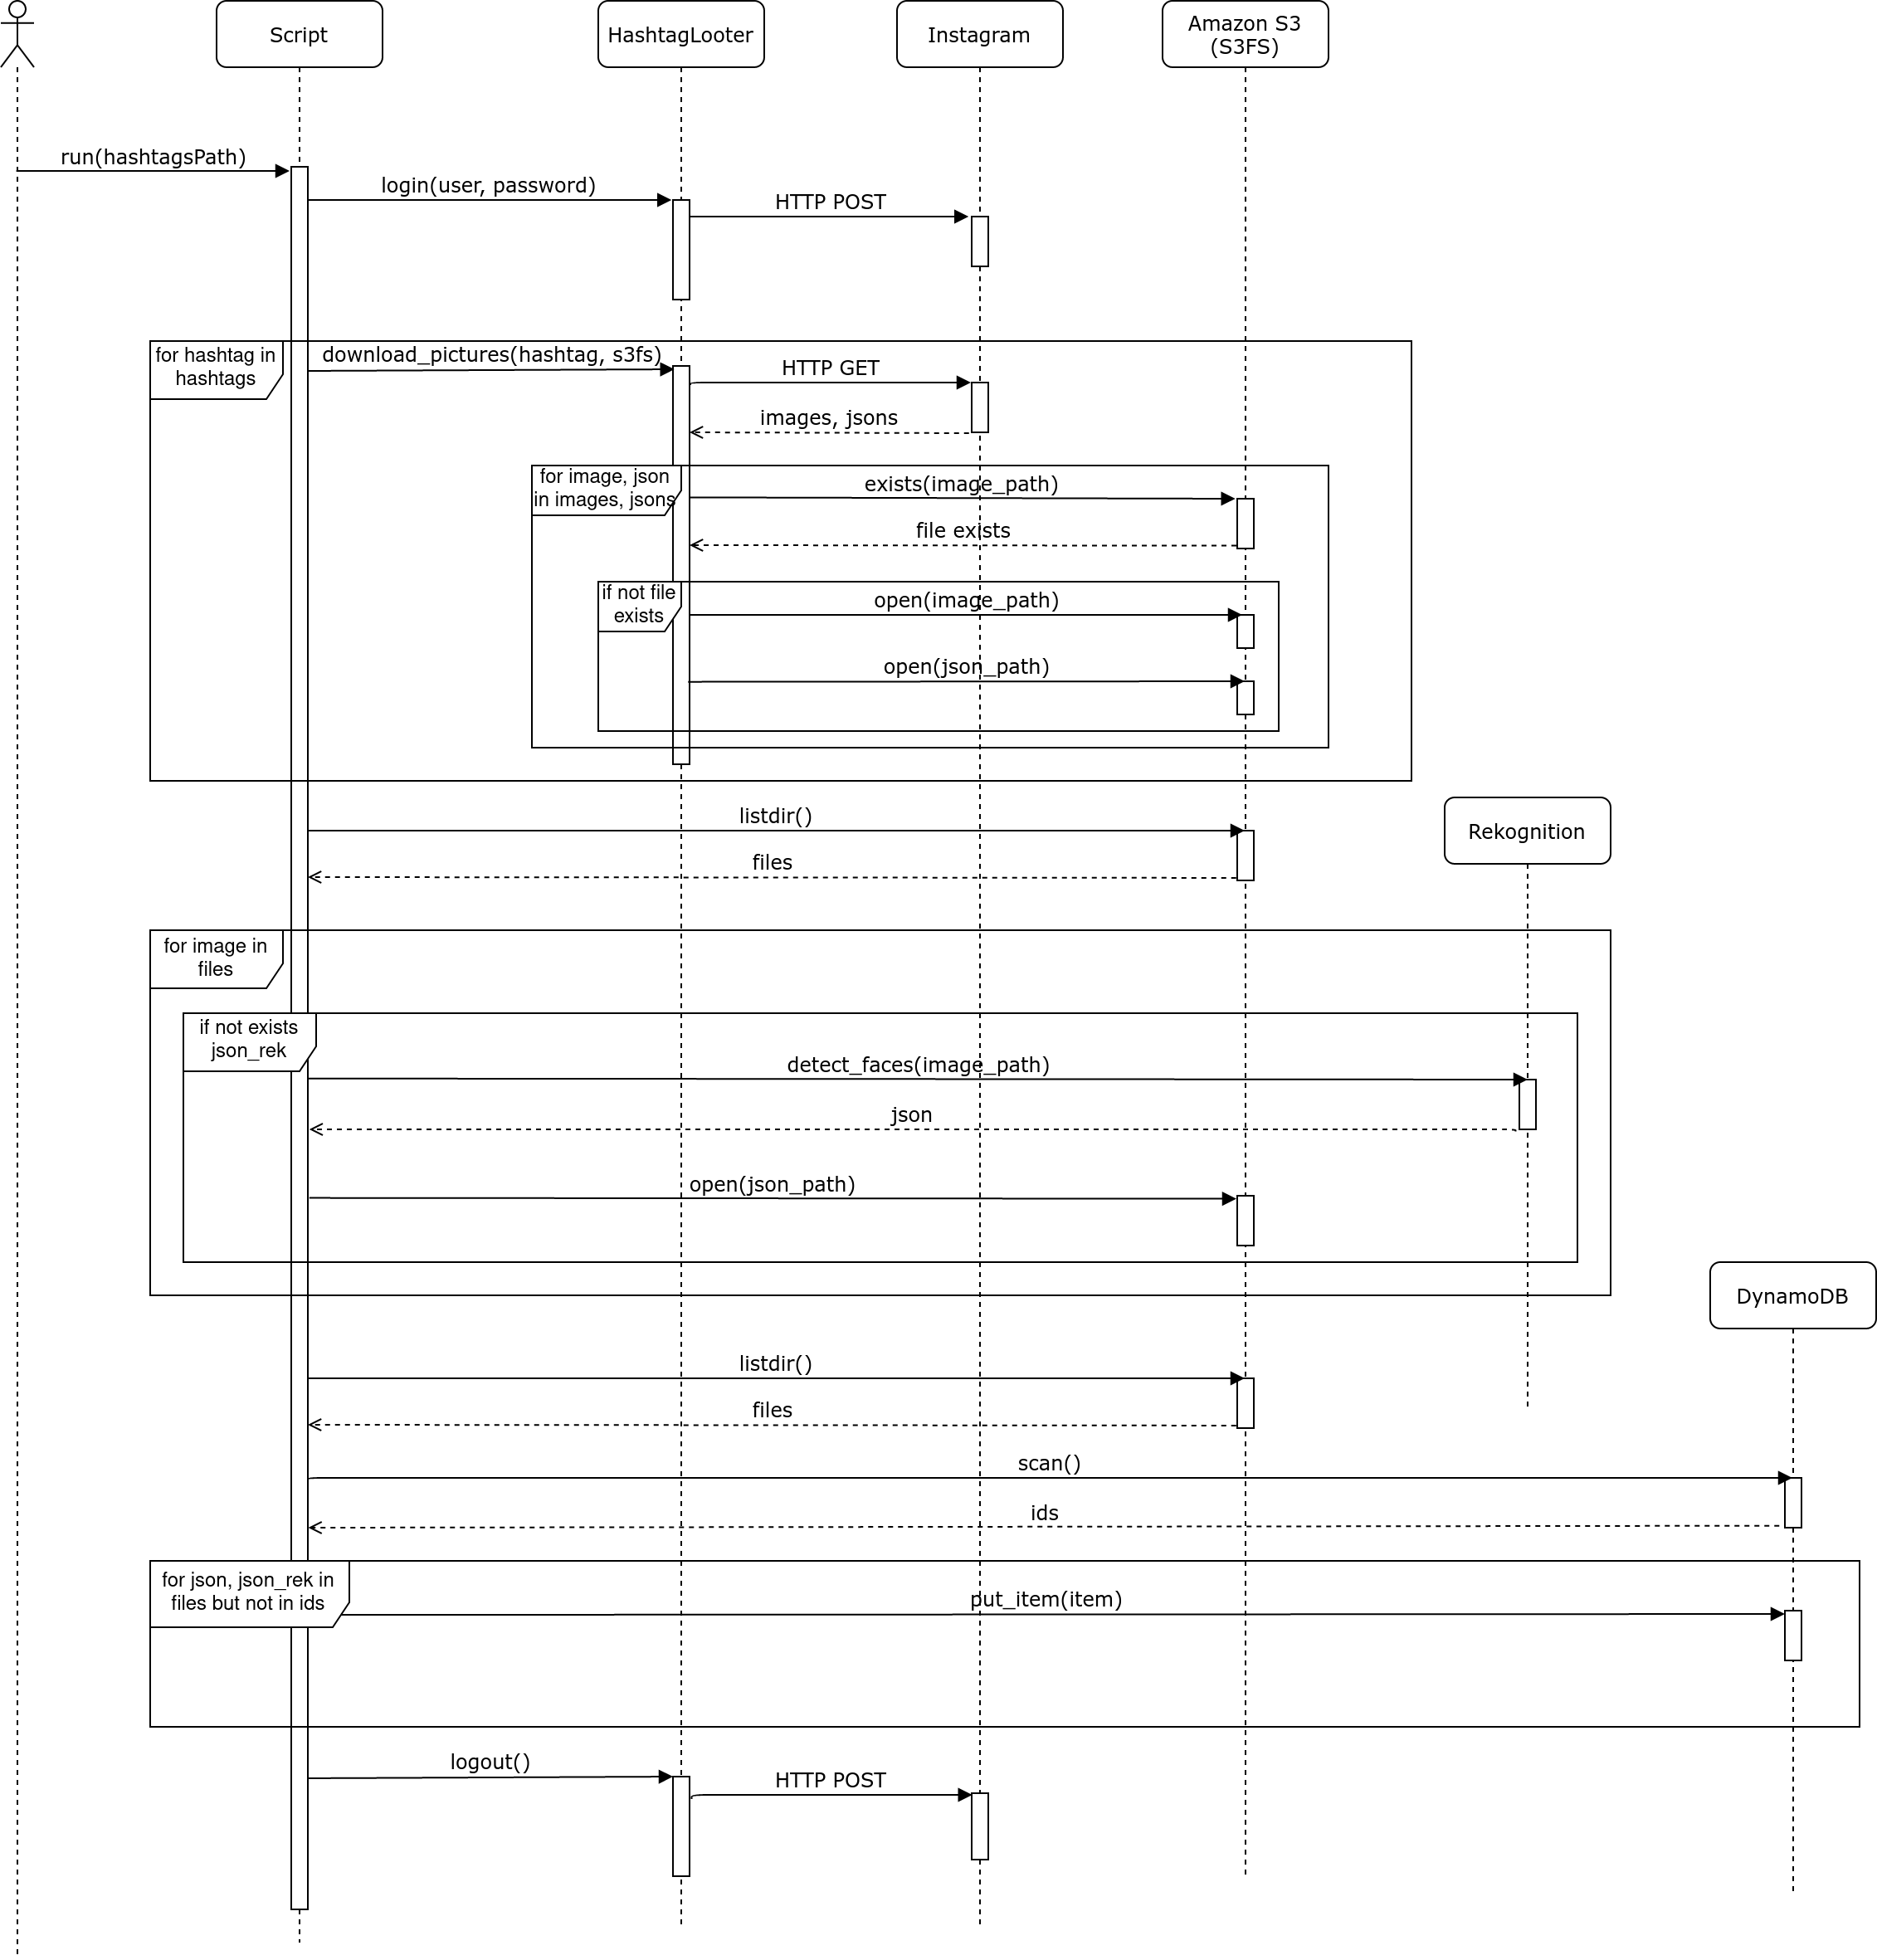
\includegraphics[width=1.25\textwidth]{sequence.drawio.png}
    \caption{Diagrama de secuencia de \texttt{mainScriptAWS.py}}
    \label{fig:sequence_script}
\end{figure}

Como se puede ver en el diagrama anterior, el script tan solo toma como argumento la ruta del fichero que contiene la lista de hashtags a consultar en Instagram (un hashtag por línea). El resto de identificadores y credenciales para acceder a Instagram o a los servicios de AWS han de estar definidos como variables de entorno.

\section{Proceso de descarga de las publicaciones}

Para llevar a cabo el proceso de descarga de publicaciones y el poblado de la base de datos se tuvo que ejecutar el script de la sección anterior en varias ocasiones. El entorno de ejecución desde el que puso en funcionamiento siempre fue una máquina virtual, con Python 3, \texttt{virtualenv} y todas las librerías y SDKs instalados. Esta maquina virtual es una de las instancias que Amazon Web Services permite crear en su capa gratuita mediante su servicio EC2. Exactamente, la configuración escogida para esta instancia es la siguiente: 1 CPU \texttt{t2.micro}, 1 GB de RAM, 30 GBs de almacenamiento SSD, 100 GBs de ancho de banda con IP estática y el sistema operativo Debian 11 de 64 bits.

Sobre la lista de hashtags que se pasa al script como argumento, inicialmente se decidió obtener un número cercano a 50 hashtags relacionados con Valladolid y el turismo en Valladolid. Esta lista habría que obtenerla manualmente buscando en Instagram hashtags populares dentro de este contexto así como las etiquetas de las publicaciones encontradas. La lista finalmente creada consta de los siguientes 44 hashtags:

\begin{multicols}{3}
\begin{itemize}
	\item Naturaleza\_valladolid
	\item estaes\_valladolid
	\item valladolidturismooficial
	\item turismovalladolid
	\item valladolidturismo
	\item turismovalladolid
	\item valladolidspain
	\item valladolidfotos
	\item valladolidenfotos
	\item valladolid
	\item todo\_valladolid
	\item total\_valladolid
	\item igersvalladolid
	\item igervalladolid
	\item catedraldevalladolid
	\item paseandoporvalladolid
	\item valladolidgram
	\item instavalladolid
	\item valladolidlove
	\item valladolidlife
	\item valladolidmola
	\item megustavalladolid
	\item fotosdevalladolid
	\item valladolidhoy
	\item vallafotos
	\item valladolidinquieta
	\item love\_valladolid
	\item visitvalladolid
	\item look\_valladolid
	\item ok\_valladolid
	\item megustavalladolid
	\item asi\_es\_valladolid
	\item pucela
	\item megustapucela
	\item arquitecturavalladolid
	\item valladolidespaña
	\item culturavalladolid
	\item valladolidcapital
	\item valladolidcampogrande
	\item valladolidpaseozorrilla
	\item iglesiadelaantiguavalladolid
	\item igerspucela
	\item rinconesdevalladolid
	\item megustapucela
\end{itemize}
\end{multicols}

A la hora de ejecutar el script un detalle a tener en cuenta es el límite de publicaciones que podemos descargar y analizar en la capa gratuita. Al mes, en Rekognition se pueden analizar hasta 5000 imágenes, en DynamoDB se tiene un límite de 200 millones de solicitudes y en S3 existe un límite de 2000 solicitudes \textit{put}, siendo este último punto el mayor factor limitante. Debido a esto y al límite de la fecha de entrega del proyecto, en la base de datos finalmente generada se descargaron un total de 3916 publicaciones de Instagram. Tras el análisis con Rekognition, a partir de estas publicaciones se extrajeron unas 5408 caras.

Un detalle a destacar fue que, durante una de las ejecuciones del script, se detectó un problema a la hora de iniciar sesión en Instagram mediante Instalooter, impidiendo llevar a cabo el proceso de descarga de publicaciones. Tras revisar el error generado por el scraper y comprobar que este no era puntual, se llegó a la conclusión de que debió de haber alguna actualización en la web de Instagram que provocó que la librería dejara de funcionar correctamente. Revisando la pestaña de problemas en el repositorio de GitHub de la librería, se observó que es un error que le sucedía a más usuarios.

Como las últimas actualizaciones del repositorio de Instalooter fueron hace varios meses en el momento en que se hizo la comprobación, se decidió probar de nuevo otras librerías como \textit{Instaloader}, pero se llegó a la conclusión de que su uso era muy distinto a Instalooter y no ofrecía las ventajas de poder comprobar publicaciones ya descargadas y poder conectarlo de forma sencilla a los servicios en la nube. Es por ello que se decidió revisar el código fuente de la librería, y tras unas pruebas se consiguió dar con la fuente del error: un cambio en como se gestionaban las \textit{cookies} donde se guardan los \textit{tokens} empleados para logearse en la web. Como el cambio no era muy complicado se decidió corregirlo en un fork \url{https://github.com/Zalez95/InstaLooter.git} de la librería, y tras comprobar que funcionaba correctamente, se instaló mediante \texttt{pip3} en el entorno de la máquina virtual. Tras está corrección no volvió a dar problemas, y de hecho se hizo un \textit{pull request} a la librería original que en la actualidad está en proceso de revisión.

\section{Visualización}

Una vez se han obtenido los datos necesarios para el proyecto, para poder usarlos de forma más cómoda se decidió que era necesario implementar algún tipo de visualización. Esta visualización debería permitir filtrar los datos de forma sencilla de acuerda a criterios como edad o género, y permitir seleccionar aquellas publicaciones que tuvieran un sentimiento positivo. También debería poder llevarnos fácilmente hasta las publicaciones mostradas en Instagram.

De acuerdo a las necesidades anteriores se llegó a la conclusión de que la forma más óptima de visualizar los datos era llevar a cabo algún tipo de cuadro de mandos. Para implementar un cuadro de mandos sobre una base de datos de DynamoDB se encontraron varias posibilidades:

\begin{enumerate}
    \item QLik: herramienta para crear dashboards con la que se ha trabajado anteriormente en este mismo máster, exactamente en la asignatura de Inteligencia de Negocio. No es una herramienta gratuita ni software libre, pero ofrece un periodo de prueba. El problema es que no se puede usar directamente con DynamoDB, sino que hay que usar un conector ODBC de la empresa Simba que no es gratuito.
    \item Microsoft PowerBI: Al igual que en la herramienta anterior, no es gratuito pero ofrece un periodo de prueba. Tampoco tiene conectores con DynamoDB, habría que usar el conector ODBC de Simba anteriormente comentado.
    \item Tableau: Ofrece un periodo de \textit{trial} de 3 meses, además existe una versión \textit{public} gratuita. Para usarlo junto con DynamoDB habría que usar el conector JDBC de Rockset que tampoco es gratuito (hay periodo de prueba pero no se indica durante cuanto tiempo).
    \item Grafana: Es open source pero no tiene conector gratuito con DynamoDB. Parece que tiene plugins que permiten conectarlo con servicios REST de forma sencilla. Se podría crear un conector creando un servidor que implementara estas APIs REST para acceder a DynamoDB como se hace en \cite{grafana_lambda_api}.
    \item Web estática junto con alguna librería para hacer gráficos: En esta opción habría que crear una página web estática manualmente y programar los gráficos en JavaScript mediante alguna librería como ChartJS o D3.js, conectándose con la base de datos a través del SDK de AWS para este lenguaje de programación. Un ejemplo de implementación se puede encontrar en \cite{web_chartjs}.
\end{enumerate}

Finalmente se decidió emplear Grafana aunque haya que implementar el conector, puesto que al ser open source no se tiene restricciones de tiempo de uso. Crear una página web estática desde cero o usando librerías consume mucho tiempo, y el resto de herramientas para hacer cuadros de mando también presentan el mismo problema a la hora de conectar con DynamoDB.

Para crear el cuadro de mandos con Grafana hubo que instalar Grafana Enterprise. En este caso se decidió hacerlo en la misma máquina virtual que se usa también para la ejecución del script de la sección anterior. Grafana es una aplicación web que por defecto se ejecuta en el puerto 3000, es por ello que para acceder desde fuera de este equipo hubo que abrir el puerto añadiendo una regla TCP en los grupos de seguridad de Amazon EC2. Una vez instalado Grafana y con el servicio corriendo, el siguiente paso fue instalar el plugin \texttt{JSON} para conectarse con fuentes de datos (\textit{data sources}) a través de HTTP. Para que este plugin funcione, el servidor al que se conecte ha de implementar una API REST con las siguientes operaciones:

\begin{itemize}
    \item \texttt{GET /} $\rightarrow$ Ha de devolver un código 200 OK si el servicio funciona correctamente.
    \item \texttt{POST /query} $\rightarrow$ Ha de devolver los valores pedidos. Para ello esta función tiene como parámetros un rango de fechas en el que se tienen que encontrar los datos, y da la posibilidad de filtrar por más valores mediante unos \textit{adhoc filters}. Los valores devueltos pueden estar en formato de tabla o en formato clave-valor, siendo la clave una fecha y el valor el contenido de una columna.
    \item \texttt{POST /search} $\rightarrow$ Ha de devolver las distintas métricas para llevar a cabo el filtrado, en nuestro caso se corresponde con el nombre de las columnas, o los posibles valores si como parámetro llega el nombre de una columna.
    \item \texttt{POST /tag-keys} $\rightarrow$ Ha de devolver las posibles claves para llevar a cabo el filtrado, en nuestro caso se corresponde con el nombre de las columnas.
    \item \texttt{POST /tag-values} $\rightarrow$ Ha de devolver los posibles valores de una clave para llevar a cabo el filtrado, en nuestro caso se corresponde con los valores distintos que hay para una columna.
\end{itemize}

Para poder crear el conector entre Grafana y DynamoDB hubo que hacer un servidor web que implementara las anteriores APIs, en este caso mediante Python 3 y el SDK de AWS \texttt{boto3}. Las pruebas iniciales se hicieron mediante un framework llamado \textit{bottle} para poder crear las APIs de forma local, y una vez que se comprobó que éstas funcionaban correctamente, se decidió implementar las APIs en Amazon Web Services para tener mejor rendimiento. Para implementar las APIs en AWS se usó sus servicios AWS Lambda, Amazon API Gateway y Amazon DynamoDB de la siguiente forma:

\begin{figure}[H]
    \centering
    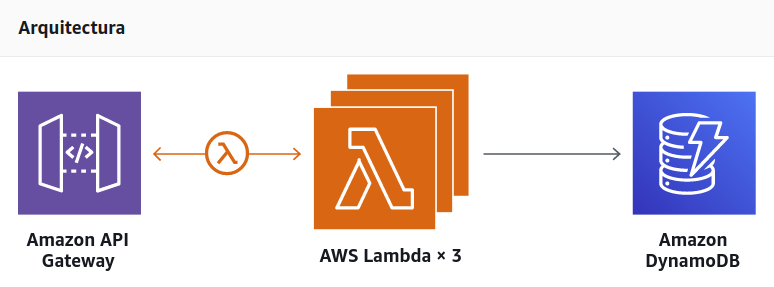
\includegraphics[width=0.9\textwidth]{gateway.png}
    \caption{Acceso a DynamoDB mediante APIs REST con API Gateway}
    \label{fig:gateway_schema}
\end{figure}

Siendo el diagrama de componentes del sistema completo el siguiente:

\begin{figure}[H]
    \hspace*{-1cm}
    \centering
    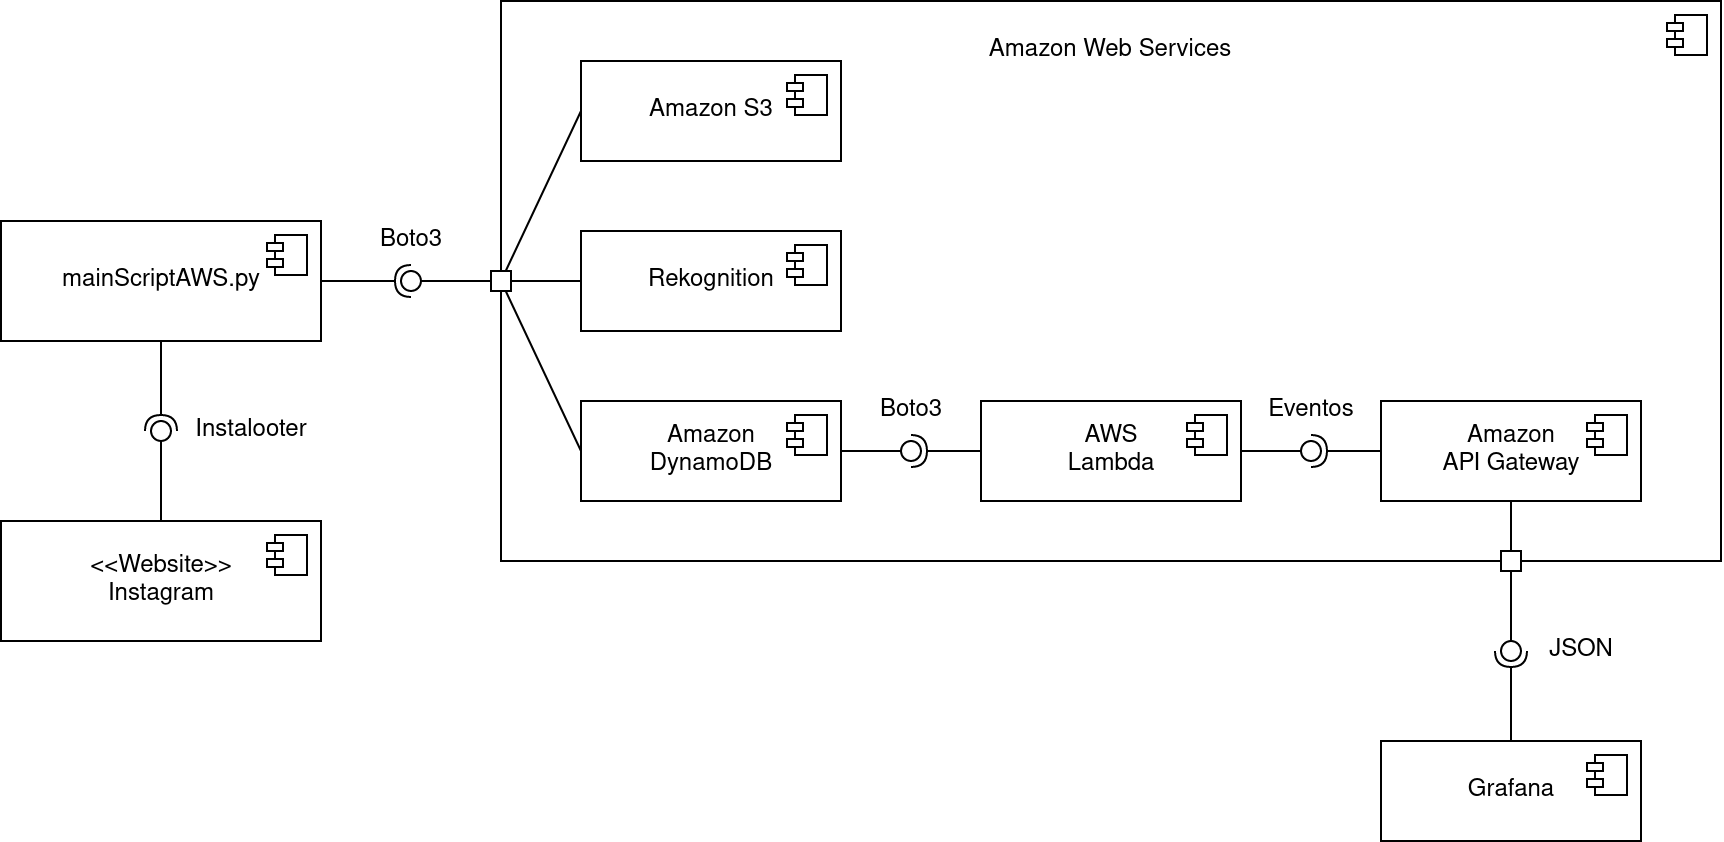
\includegraphics[width=1.2\textwidth]{memoria/img/component.drawio.png}
    \caption{Diagrama de Componentes del sistema}
    \label{fig:component_diag}
\end{figure}

AWS Lambda permite ejecutar código en la nube de Amazon sin tener que crear instancias de máquinas virtuales. En total se generaron 5 funciones para acceder a DynamoDB: \texttt{grafana\_query}, \texttt{grafana\_tagkeys}, \texttt{grafana\_helloworld}, \texttt{grafana\_tagvalues}, \texttt{grafana\_search}, implementando el acceso a DynamoDB y la lógica correspondiente. Todas estas funciones se ejecutan en un entorno Python 3.8 en equipos x86\_64, con un tiempo de ejecución de máximo 1 minuto. Por otro lado, API Gateway es el servicio que permite implementar de forma sencilla y escalable APIs RESTful o Websocket. En este caso las APIs REST se generaron como recursos que tienen asociado un método HTTP y un \textit{endpoint}, y que al ser accedidas ejecutan su correspondiente función de AWS Lambda:

\begin{figure}[H]
    \hspace*{-2cm}
    \centering
    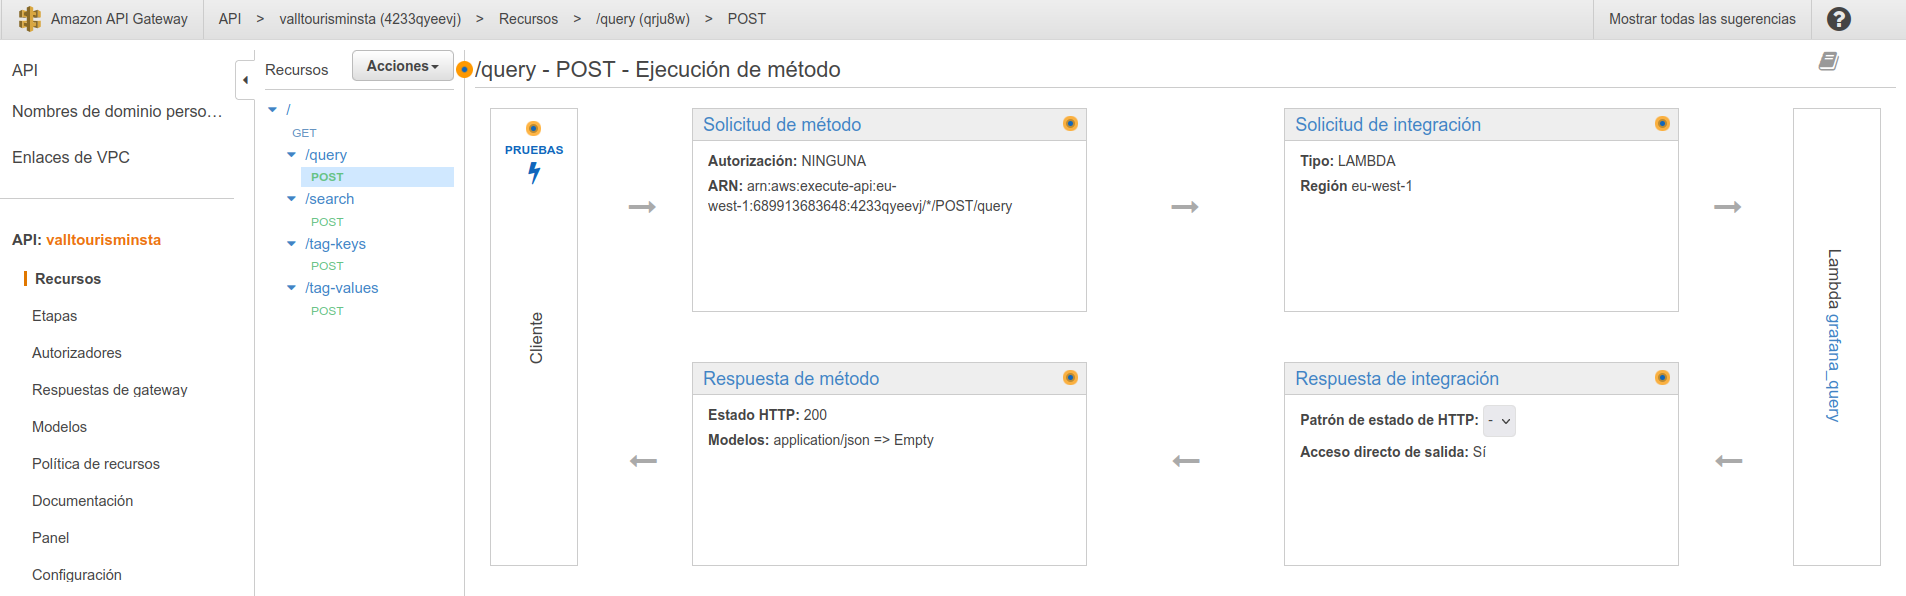
\includegraphics[width=1.25\textwidth]{gateway_cap.png}
    \caption{Configuración de AWS API Gateway y AWS Lambda}
    \label{fig:gateway_cap}
\end{figure}

Una vez que se crearon las APIs, el siguiente paso fue emplearlas con Grafana. Para ello se generó un \textit{data source} de tipo JSON que apuntaba a la URL del servicio de API Gateway. Tras conectar con éxito con la fuente de datos se procedió a la implementación del cuadro de mandos.

Para el diseño del dashboard se decidió emplear 3 columnas y 2 filas, ubicándose la información más relevante en la esquina superior izquierda puesto que está probado que las personas siguen un patrón en forma de Z a la hora visionar documentos o cuadros de mandos. El resultado final se puede ver en la figura \ref{fig:dashboard}.

En la esquina superior izquierda se muestra una combinación de estadísticas generales de las publicaciones mostradas, entre las que se encuentra el número de publicaciones mostradas, el número de caras y la proporción de genero de las caras mediante un gráfico de tarta. A su derecha se encuentra una tabla con información condensada de cada publicación, con un enlace hacia la publicación en Instagram, su fecha, la confianza, el género y la edad. Después, en la esquina superior derecha se muestra el número de publicaciones por fecha en un histograma para así poder ver que días hubo más publicaciones.

En la siguiente fila se muestra, a la izquierda la emoción predominante en todas las publicaciones, para ello se calcula el promedio de la confianza de cada emoción de todas las publicaciones y se muestra en un gráfico de tarta. A su derecha, el ``éxito'' de las publicaciones, en un histograma que muestra el promedio del número de comentarios y de likes que hubo cada día. Finalmente a su derecha se muestra la emoción promedio de las publicaciones por día.

\begin{figure}[H]
    \hspace*{-2.5cm}
    \centering
    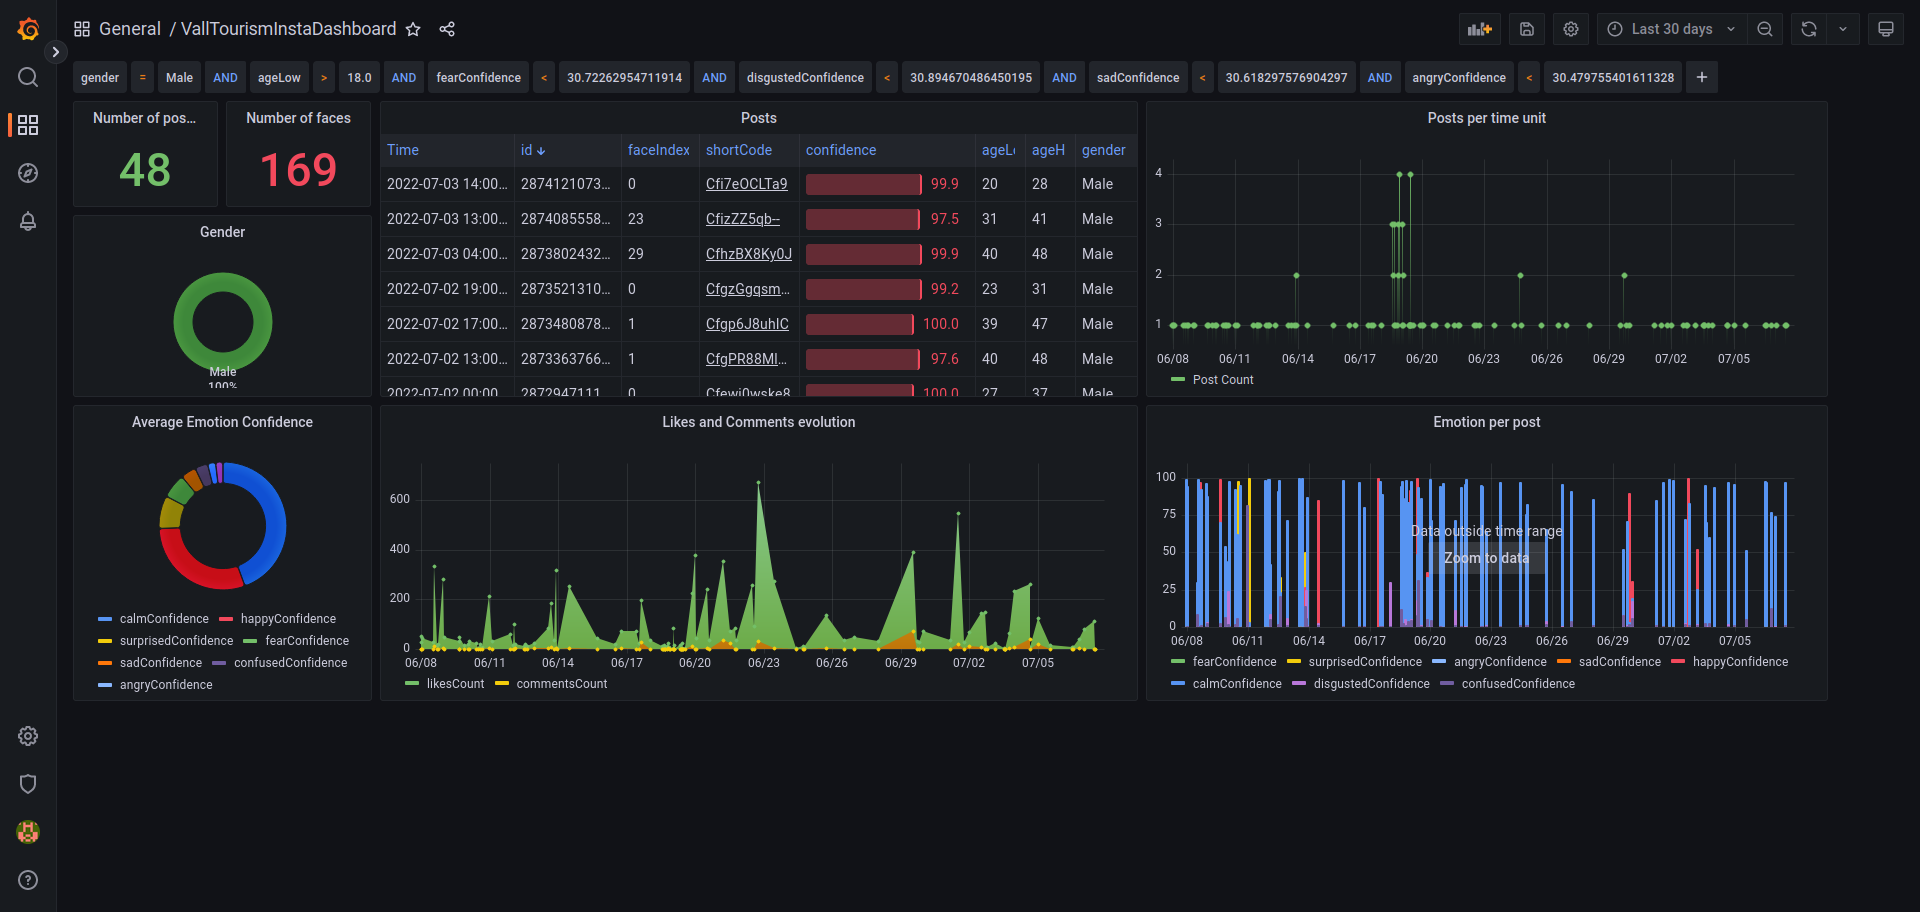
\includegraphics[width=1.3\textwidth]{dashboard.png}
    \caption{Cuadro de Mandos creado con Grafana}
    \label{fig:dashboard}
\end{figure}

Cabe destacar que Grafana muestra en la parte superior los distintos filtros a aplicar, por un lado las fechas, y por otro los filtros \textit{adhoc}, que pueden ser añadidos o modificados dinámicamente. En la captura anterior se puede ver que se están mostrando los últimos 30 días, y que se tienen habilitados varios filtros, exactamente género masculino, edad superior a los 18 años y se ha intentado que no haya emociones negativas predominantemente, descartando aquellas publicaciones que tengan una confianza superior al 30\% aproximadamente en las emociones triste, enfadado y disgustado.

\capitulo{6}{Trabajos relacionados}

En este apartado se va a exponer el estado del arte, o los trabajos encontrados relacionados con el tema del presente proyecto con el fin de conocer si ya existe algún trabajo anterior que intente resolver el mismo problema que el aquí presentado.\\

\subsection{Metodología de trabajo}

Durante este proceso de documentación, lo primero que se llevó a cabo fue una búsqueda preliminar con el fin de conocer si existía algún artículo previo donde se tratara en específico el análisis de emociones en imágenes de Instagram para recomendar posts o lugares a los que visitar. Para ello se hizo uso de bases de datos y exploradores gratuitos como Google Scholar, IEEE Xplore y ResearchGate. El resultado de esta búsqueda fue negativo, pero sí que se encontraron multitud de trabajos en los que se intentaba llevar a cabo análisis de sentimiento de comentarios de diversas redes sociales para saber la reacción de los usuarios que hacían turismo en cierto lugares en específico como \cite{8720960}, o trabajos generales sobre análisis de sentimiento para ayudar a recomendadores como \cite{techniques_media_based_recom} o \cite{recom_sys_sen_analysis}.\\

Como este trabajo preliminar no fue satisfactorio, se decidió ampliar los criterios de búsqueda, llevando a cabo un proceso de \textit{map-review} con el objetivo de recopilar los trabajos previos más relevantes para el presente proyecto. Debido a que la cantidad de artículos relacionados con análisis de sentimiento es abrumadora, para llevar a cabo el map-review se decidió emplear la metodología PRISMA (\textit{Preferred Reporting Items for Systematic Reviews and Meta-Analyses}) inspirado por el artículo \cite{recom_metodo_tutor}. Esta metodología es empleada para llevar a cabo revisiones sistemáticas de conjuntos de artículos, permitiendo descartar aquellos que no son relevantes sin tener que leerlos todos por completo, agilizando todo el proceso. En resumen, esta metodología cuenta de varias etapas:

\begin{enumerate}
    \item Planificación de búsqueda: Hay que comprobar que no haya ya un trabajo previo que resuelva la misma pregunta. En nuestro caso como se comentó al inicio del apartado, aparentemente no parece haber un trabajo anterior similar.
    \item Proceso de búsqueda: En esta fase hay que generar las cadenas de búsqueda que se emplearan en los buscadores de artículos. En nuestro caso se decidió emplear las siguientes cadenas:
    \begin{itemize}
        \item \texttt{(Sentiment Analysis OR Emotion Recognition) AND Social Media AND Tourism}
        \item \texttt{(Sentimen Analysis OR Emotion Recognition) AND Images \\
        AND Recommendation System}
    \end{itemize}
    
    Además de las anteriores cadenas de búsqueda, se ha decidido también aplicar otros filtros a mayores como:
    
    \begin{itemize}
        \item El acceso al artículo se ha de poder hacer de forma gratuita.
        \item El artículo ha de ser ``actual'', de entre 2014 y 2022.
    \end{itemize}
    
    De este modo se obtuvieron un total de 22 artículos a analizar en las siguientes fases.

    \item Selección de muestras. En esta fase se parte de los artículos anteriormente obtenidos y, tras descartar aquellos que estén duplicados, se decide si descartar alguno tras leer el \textit{abstract} basándose en una serie de criterios de inclusión y de exclusión. En este caso se ha decidido que:

    \begin{itemize}
        \item Se incluye si:
        \begin{itemize}
            \item El abstract está relacionado con análisis de sentimientos en redes sociales
            \item El abstract está relacionado con análisis de sentimientos en imágenes
            \item El abstract está relacionado con sistemas de recomendación de turismo
        \end{itemize}
        
        \item Se excluye si :
        \begin{itemize}
            \item El idioma del artículo no es inglés ni español.
            \item El artículo no se puede acceder gratuitamente
            \item El artículo es una recopilación de trabajos previos
            \item El artículo no está relacionado con análisis de sentimientos
            \item La fuente de datos del artículo no son redes sociales
        \end{itemize}
    \end{itemize}

    Si tras leer el abstract es detectado algún criterio de exclusión o no cumple con ningún criterio de inclusión, el artículo es directamente es descartado. Después de descartar por el abstract, los artículos restantes son leídos por completo y se decide si incluirlos o no basándose en un test con las siguientes preguntas binarias (Sí o No):

    \begin{enumerate}
        \item ¿Emplea herramientas de análisis de sentimientos?
        \item ¿Emplea análisis de sentimiento basado en imágenes?
        \item ¿Emplea análisis de sentimiento en redes sociales?
        \item ¿Hace referencia a sistemas de recomendación de turismo?
        \item ¿Contiene tablas y gráficos de resultados?
    \end{enumerate}
    
    Solo son aceptados aquellos artículos que superen el anterior test con 3 sí-es. Tras este proceso de cribado se llegó a la conclusión de que solo 6 de los 22 trabajos considerados anteriormente eran relevantes para el nuestro.
\end{enumerate}

De los trabajos finalmente considerados, estos podrían ser divididos en tres categorías: por un lado tenemos los trabajos donde se busca recomendar contenido, posts o usuarios que seguir, por otro lado, tenemos trabajos donde se recomiendan lugares que visitar, y por último tenemos trabajos donde se busca analizar las opiniones sobre un destino turístico.\\

\subsection{Recomendación de contenido}

Dentro del primer grupo encontramos trabajos como \cite{sent_analysis_facebook_user_recom} donde se investiga el uso de análisis de sentimiento en la red social Facebook para mejorar los resultados de las recomendaciones de usuarios/amigos. Para llevar a cabo este objetivo, en este trabajo se analiza el texto de las publicaciones de los usuarios para extraer conceptos de las mismas, la subjetividad u objetividad de las frases, y los sentimientos encontrados en los documentos. A la hora de recomendar o no a un usuario, en este artículo se propone una novedosa función de peso que tiene en cuenta el sentimiento de un usuario hacia un concepto así como el número de publicaciones de tal usuario acerca del mismo. La evaluación del método propuesto se hizo empleando un conjunto de datos de más de 6 millones de publicaciones extraídas de Facebook, dando un resultado superior a otros métodos ya establecidos.\\

Por otro lado, también encontramos trabajos como \cite{pers_tweet_recomendation}, donde se propone un sistema de recomendación de \textit{tweets} personalizado dentro del dominio de la salud. Para ello hace uso del análisis de sentimiento para la creación de un perfil de usuario basándose en el historial en la red social del usuario. El sistema propuesto consta de dos módulos, el primero se encarga de generar un perfil de usuario mediante la extracción información de su cuenta, sus intereses en temas de salud y los patrones de emoción a lo largo del tiempo, mientras que el segundo recoge datos públicos de Twitter, lleva a cabo un procesamiento de lenguaje natural y los clasifica para poder recomendarlos a los usuarios basándose en su correspondiente perfil. Este sistema se probó contra casi 1 millón de \textit{tweets} de distintas categorías, alcanzando una precisión del 96\%.\\

\subsection{Recomendación de lugares}

Dentro del segundo grupo existen trabajos como \cite{8796367} donde se presenta un sistema de recomendación de turismo personalizado teniendo en cuenta las preferencias del usuario. Su método denominado SMTM divide el problema en dos dominios, por un lado la extracción de los tópicos relacionados con una atracción turística, y por otro las preferencias del turista respecto a las atracciones a partir de textos e imágenes. Por último trata de proyectar los resultados del dominio del turista en el dominio de la atracción. Para probar el modelo generado con otros modelos se emplearon dos datasets, el primero generado a partir de de información del portal web TripAdvisor, y el segundo a partir de datos de la web Trip, en ambos casos los resultados obtenidos fueron mejores que el resto de métodos comparados.\\

Además, también tenemos el trabajo \cite{recom_mech_under_emph} donde se propone un sistema de recomendación de turismo con dos objetivos, primero satisfacer las expectativas del turista, y segundo ayudar a las agencias de marketing a orientar sus promociones. Este sistema de recomendación se planteó con el objetivo de poder recomendar tanto lugares altamente valorados como aquellos que son pasados por alto por muchos turistas pero que merecen la pena, a los que llama lugares poco enfatizados, y cabe destacar que este sistema de recomendación es personalizado, teniendo en cuenta el historial del usuario. El sistema consta de varios módulos, el primero se usa para llevar a cabo una extracción de tópicos de las reviews publicadas en Google y en TripAdvisor. El segundo lleva a cabo un análisis de sentimiento mediante máquinas de vectores soporte. Por último emplea una red neuronal artificial para recomendar los lugares a los usuarios, empleando una función de optimización para conseguir el objetivo de recomendar lugares poco enfatizados. Para probar el sistema se empleó un dataset con casi 150.000 publicaciones, llegando a obtener tener una precisión del 94\%.\\

\subsection{Análisis sobre destinos turísticos}

A diferencia de los trabajos anteriores donde el objetivo era el estudio o creación de sistemas de recomendación, existen trabajos como \cite{tourism_dest_rec_geolocation} donde se compara el rendimiento de múltiples métodos actuales de aprendizaje profundo con el fin de llevar a cabo un análisis de sentimiento de los tweets relacionados con Cilento, un popular destino turístico del sur de Italia. En este artículo se llegan a comparar 4 tipos de redes neuronales profundas empleando un dataset de casi 20000 tweets en inglés e italiano, cuyo sentimiento tuvo que ser clasificado manualmente de forma previa. Además de la comparación de estos métodos, en dicho artículo consiguen generar un mapa mediante la geolocalización de los tweets para poder así visualizar el sentimiento promedio en ciertas regiones del municipio.\\

También en \cite{su13116015} se lleva a cabo un análisis sobre el turismo en España y la percepción que tienen los turistas chinos empleando publicaciones en portales y redes sociales de China con el objetivo de medir la calidad de los distintos destinos turísticos. Para ello obtuvieron una dataset de casi 40 mil publicaciones, y llevaron a cabo una extracción de tópicos relacionados con las publicaciones así como análisis de sentimientos mediante procesamiento de lenguaje natural.\\
\capitulo{7}{Conclusiones y Líneas de trabajo futuras}

%Todo proyecto debe incluir las conclusiones que se derivan de su desarrollo. Éstas pueden ser de diferente índole, dependiendo de la tipología del proyecto, pero normalmente van a estar presentes un conjunto de conclusiones relacionadas con los resultados del proyecto y un conjunto de conclusiones técnicas. 
%Además, resulta muy útil realizar un informe crítico indicando cómo se puede mejorar el proyecto, o cómo se puede continuar trabajando en la línea del proyecto realizado. 

En este apartado se presentan las conclusiones finalmente obtenidas del desarrollo del proyecto, así como posibles mejoras o alternativas a desarrollar en el futuro.

\section{Conclusiones}


El desarrollo de la base de datos final ha estado más limitado de lo esperado debido al máximo número de elementos que se pueden meter en Amazon S3 en su capa gratuita.

Los crawlers son muy sensibles a las actualizaciones de las páginas web, y teniendo en cuenta la popularidad de Instagram y la frecuencia de sus actualizaciones los fallos son comunes.

Dentro de los objetivos personales planteados al inicio del proyecto cabe destacar que finalmente si que se ha conseguido explorar múltiples herramientas.

\section{Líneas de trabajo futuras}



%\renewcommand\chaptername{Anexo}
%\renewcommand\thechapter{\Roman{chapter}}
%\setcounter{chapter}{0}

% Añadir entrada en el índice: Anexos
\appendix
\addcontentsline{toc}{part}{Apéndices}
\part*{Apéndices}

\apendice{Plan de Proyecto Software}

\section{Introducción}

En este apartado se presenta la planificación temporal del proyecto empleando la metodología SCRUM, así como la viabilidad del proyecto desde el punto de vista legal y económico.

\section{Planificación temporal}

Como se ha indicado en el apartado anterior, para el desarrollo del proyecto se siguió la metodología \textit{SCRUM}, adaptándola a las necesidades y al tiempo disponible. Las características a destacar de esta metodología son las siguientes:

\begin{itemize}
    \item Desarrollo iterativo e incremental que permite adaptarse a cambios inesperados en los requerimientos o herramientas.
    \item El proyecto se subdivide en múltiples tareas, que se abordan a lo largo de varias iteraciones denominadas \textit{sprints}.
    \item Todos los \textit{sprints} tienen una duración prefijada, en este caso de 2 semanas.
    \item Todo \textit{sprint} se inicia o finaliza con una reunión con el tutor del proyecto.
\end{itemize}

\subsection{Sprint 0}
Durante el \textit{sprint 0} se abordaron las tareas requeridas para la inicialización del proyecto, así como la evaluación y la toma de decisión de las distintas herramientas que se pretendían utilizar durante el posterior desarrollo.

\begin{table}[H]
    \centering
    \begin{tabular}{l}
    \hline
    \textbf{Tareas} \\ \hline
    Creación del repositorio del proyecto \\
    Creación del entorno de trabajo \\
    Evaluación de la forma de extraer hashtags de Instagram \\
    Evaluación de los distintos \textit{crawlers} y herramientas a utilizar \\
    Registro y experimentación con las herramientas de Google Cloud \\ \hline
    \end{tabular}
    \caption{Tareas del \textit{sprint 0}}
    \label{tab:tasks_sprint0}
\end{table}

\subsection{Sprint 1}
Durante el \textit{sprint 1} se abordaron las tareas relacionadas con la descarga de publicaciones de Instagram y se inició el desarrollo de la memoria.

\begin{table}[H]
    \centering
    \begin{tabular}{l}
    \hline
    \textbf{Tareas} \\ \hline
    Creación de la máquina virtual \\
    Implementación de la descarga de publicaciones mediante Instalooter \\
    Subida de publicaciones a un \textit{blob} de Google Cloud \\
    Pruebas de reconocimiento facial con Cloud Vision \\
    Documentación sobre la metodología PRISMA para map-review \\
    Inicio de la memoria en Overleaf \\ \hline
    \end{tabular}
    \caption{Tareas del \textit{sprint 1}}
    \label{tab:tasks_sprint1}
\end{table}

\subsection{Sprint 2}
Durante el \textit{sprint 2} se evaluaron las alternativas a Cloud Vision tras comprobar que no se podía extraer la edad ni el género. También se redactó la parte de trabajos relacionados o el estado del arte de la memoria.

\begin{table}[H]
    \centering
    \begin{tabular}{l}
    \hline
    \textbf{Tareas} \\ \hline
    Evaluación de las alternativas a Cloud Vision y Google Cloud \\
    Pruebas con Microsoft Azure \\
    Pruebas con Amazon Web Services \\
    Elección de los artículos relacionados \\
    Redacción del apartado de Trabajo relacionados \\ \hline
    \end{tabular}
    \caption{Tareas del \textit{sprint 2}}
    \label{tab:tasks_sprint2}
\end{table}

\subsection{Sprint 3}
Durante el \textit{sprint 3} se decidió emplear Amazon Web Services tras comprobar que era la mejor alternativa. Se llevaron a cabo los cambios en los scripts y se implementó la descarga de datos de reconocimiento facial.

\begin{table}[H]
    \centering
    \begin{tabular}{l}
    \hline
    \textbf{Tareas} \\ \hline
    Adaptación de los scripts para usar los servicios de Amazon \\
    Implementación de la descarga de datos de reconocimiento facial \\
    Evaluación de las posibles bases de datos a utilizar \\
    Evaluación de las posibles visualizaciones a implementar \\ \hline
    \end{tabular}
    \caption{Tareas del \textit{sprint 3}}
    \label{tab:tasks_sprint3}
\end{table}

\subsection{Sprint 4}

Durante el \textit{sprint 4} se diseñó e implementó la base de datos en DynamoDB. También se tuvo que llevar a cabo una corrección en Instalooter después de que dejara de funcionar.

\begin{table}[H]
    \centering
    \begin{tabular}{l}
    \hline
    \textbf{Tareas} \\ \hline
    Diseño e implementación de la base de datos \\
    Implementación de los scripts de subida de datos a DynamoDB \\
    Hotfix de Instalooter \\
    Evaluación de los posibles dashboards a utilizar \\ \hline
    \end{tabular}
    \caption{Tareas del \textit{sprint 4}}
    \label{tab:tasks_sprint4}
\end{table}

\subsection{Sprint 5}

Durante el \textit{sprint 5} se tomó la decisión de implementar un cuadro de mandos con Grafana, por ello se iniciaron las pruebas para crear un conector con DynamoDB, también se finalizó el script para poblar la base de datos.

\begin{table}[H]
    \centering
    \begin{tabular}{l}
    \hline
    \textbf{Tareas} \\ \hline
    Creación del script final de descarga y subida de datos a DynamoDB \\
    Llenado de la base datos \\
    Pruebas con Grafana \\
    Desarrollo de un servidor local para conectar Grafana con DynamoDB \\ \hline
    \end{tabular}
    \caption{Tareas del \textit{sprint 5}}
    \label{tab:tasks_sprint5}
\end{table}

\subsection{Sprint 6}

Durante el \textit{sprint 6} se finalizó el conector de Grafana con DynamoDB, se implementó el cuadro de mandos final y se continuó con la redacción de la memoria.

\begin{table}[H]
    \centering
    \begin{tabular}{l}
    \hline
    \textbf{Tareas} \\ \hline
    Portado del conector de Grafana a AWS Lambda y Amazon API Gateway \\
    Diseño e implementación final del Dashboard \\
    Redacción del apartado de Objetivos del proyecto \\
    Redacción del apartado de Conceptos teóricos \\
    Redacción del apartado de Técnicas y herramientas \\ \hline
    \end{tabular}
    \caption{Tareas del \textit{sprint 6}}
    \label{tab:tasks_sprint6}
\end{table}

\subsection{Sprint 7}

Durante el \textit{sprint 7} se finalizó la memoria y se reorganizó el repositorio de cara a la entrega final.

\begin{table}[H]
    \centering
    \begin{tabular}{l}
    \hline
    \textbf{Tareas} \\ \hline
    Redacción del apartado de Introducción \\
    Redacción del apartado de Aspectos relevantes del desarrollo del proyecto \\
    Redacción del apartado de Conclusiones y líneas de trabajo futuras \\
    Redacción de los apéndices \\ \hline
    \end{tabular}
    \caption{Tareas del \textit{sprint 7}}
    \label{tab:tasks_sprint7}
\end{table}

\section{Estudio de viabilidad}

\subsection{Viabilidad económica}

\subsection{Viabilidad legal}



\apendice{Especificación de Requisitos}

\section{Introducción}

\section{Objetivos generales}

\section{Catalogo de requisitos}

\section{Especificación de requisitos}



\apendice{Especificación de diseño}

\section{Introducción}

\section{Diseño de datos}

\section{Diseño procedimental}

\section{Diseño arquitectónico}



\apendice{Documentación técnica de programación}

\section{Introducción}

\section{Estructura de directorios}

\section{Manual del programador}

\section{Compilación, instalación y ejecución del proyecto}

\section{Pruebas del sistema}

\apendice{Documentación de usuario}

\section{Introducción}

\section{Requisitos de usuarios}

\section{Instalación}

\section{Manual del usuario}





\bibliographystyle{plain}
\bibliography{bibliografia}

\end{document}
